%& -output-directory=./pdf -aux-directory=./temp
%
% NOTE This requires LaTeX (SEE THAT POPUP IN THE TexShop toolbar!!!!)
% 
\documentclass[11pt,oneside]{book}
\usepackage[a4paper,left=3cm,right=2cm,top=3cm,bottom=2cm]{geometry}  
% To create the HTML pages
% 1. Uncomment on of the following lines for html generation, comment out both for pdf
%\usepackage[html,png,2,frames]{tex4ht}             
%\usepackage[html,png]{tex4ht}   
% 2. Set Typeset option TeX / Ghostscript         
% 3. execute from command line following:
% ht latex root 
%
% ht, tex4ht installed with Fink (IIRC)
%
\renewcommand{\familydefault}{\sfdefault}
\usepackage{array}
%\usepackage[draft]{graphicx}
\usepackage{graphicx}
\usepackage{amssymb,amsmath,textcomp,gensymb}
\usepackage{epstopdf}
\usepackage{alltt} 
\usepackage{threeparttable}
\usepackage[colorlinks=true,urlcolor=blue,bookmarks=true]{hyperref}
\usepackage{pdfpages}
\usepackage{pdflscape}
\usepackage[Q=yes,div=yes,bsdiv=yes]{examplep}
\usepackage{longtable}
\usepackage{listings}
\usepackage{floatflt}
\usepackage[T1]{fontenc}
\usepackage[justification=centering]{caption}
\usepackage{fancyvrb}
\usepackage{float}
\usepackage{framed}
\usepackage{hyperref}
\usepackage{wrapfig}
\usepackage{lipsum}  
\usepackage{longtable}
\usepackage{comment}
\usepackage{url}
\usepackage[defaultlines=4,all]{nowidow}


\usepackage[framemethod=TikZ]{mdframed}

\mdfdefinestyle{warning}{%
    linecolor=black,
    outerlinewidth=1pt,
    innertopmargin=\baselineskip,
    innerbottommargin=\baselineskip,
    innerrightmargin=20pt,
    innerleftmargin=20pt,
    fontcolor=red}

 \mdfdefinestyle{nobreak}{%
      outerlinewidth=0pt,
    nobreak=true}

 
\usepackage[T1]{fontenc}
\usepackage[urw-garamond]{mathdesign}
%\usepackage{garamondx}

\usepackage[section]{placeins}
%\usepackage[subsection]{placeins}





%%%%%%%%%%%%%%%%%%%%

\usepackage{lipsum}
\usepackage{mwe}

\newsavebox\iconbox
\savebox\iconbox{}
\newcommand{\seticons}[1]{%
  \savebox\iconbox{{\makebox[\iconboxwidth]{\includegraphics[width=\iconboxwidth]{#1}}}}}
\newlength{\iconboxwidth}
\setlength{\iconboxwidth}{0.5in}
\newlength{\iconsep}
\setlength{\iconsep}{4pt}
\makeatletter
\renewcommand{\@seccntformat}[1]{%
  \llap{\parbox[t][0pt]{\iconboxwidth}{\hfill{\csname the#1\endcsname}\\[\iconsep]\usebox{\iconbox}}\hspace{0.5em}}}
\renewcommand{\section}{\@startsection{section}{1}{\z@}
    {-4ex \@plus -1ex \@minus -.4ex}
    {1ex \@plus.2ex }
    {\normalfont\large\sffamily\bfseries}}
\renewcommand{\subsection}{\@startsection {subsection}{2}{\z@}
    {-3ex \@plus -0.1ex \@minus -.4ex}
    {0.5ex \@plus.2ex }
    {\normalfont\sffamily\bfseries}}

%%%%%%%%%%%%%%%%%%%% 




% -----------------------------------------------------
\begin{document}
\newcommand{\HRule}{\rule{\linewidth}{0.5mm}}
\DeclareGraphicsRule{.tif}{png}{.png}{`convert #1 `dirname #1`/`basename #1 .tif`.png}
\graphicspath{ {./images/} {./screencaps/}} 

% -----------------------------------------------------
% Here it is: the code that adjusts justification and spacing around caption.
\makeatletter
% http://www.texnik.de/floats/caption.phtml
% This does spacing around caption.
\setlength{\abovecaptionskip}{6pt}   % 0.5cm as an example
\setlength{\belowcaptionskip}{6pt}   % 0.5cm as an example
% This does justification (left) of caption.
\long\def\@makecaption#1#2{%
  \vskip\abovecaptionskip
  \sbox\@tempboxa{#1: #2}%
  \ifdim \wd\@tempboxa >\hsize
    #1: #2\par
  \else
    \global \@minipagefalse
    \hb@xt@\hsize{\box\@tempboxa\hfil}%
  \fi
  \vskip\belowcaptionskip}
\makeatother

% This causes empty line between paragraphs
\setlength{\parskip}{\baselineskip}


% -----------------------------------------------------
% Tables in courier
\makeatletter
\renewenvironment{table}%
  {\renewcommand{\familydefault}{\ttdefault}\selectfont
  \@float{table}}
  {\end@float}
\makeatother
%-------------------------------------------------------


%---------------------------------------------------------------------------
\newcommand{\screencap}[2] {
\begin{figure}[htb] 
\includegraphics[scale=0.2]{#1.png}
\caption{#2}
\label{fig:#1}
\end{figure}
Figure~\ref{fig:#1}
}
%---------------------------------------------------------------------------
\newcommand{\screencaps}[3] {
\begin{figure}[htb] 
\includegraphics[scale=#2]{#1.png} 
\caption{#3}
\label{fig:#1}
\end{figure}
Figure~\ref{fig:#1}
}
%---------------------------------------------------------------------------

% no first line indents
\setlength{\parindent}{0pt}





\begin{titlepage}
\begin{center}

\textsc{\LARGE SpareTimeLabs}\\[1.5cm]


\begin{center} \large
eazycnc@eazycnc.com
\end{center}

% Upper part of the page

\HRule \\[0.4cm]

{ \huge \bfseries EazyCNC -- Manual}\\[0.8cm]
\begin{center} 
Revision 2 
\end{center}

\begin{center}  
for 
\end{center}

\begin{center} \large
EazyCNC version 2.0.42
\end{center}

\HRule \\[0.4cm]

\includegraphics[scale=0.3]{images/title-picture.png}

\HRule \\[1.5cm]

\vfill

% Bottom of the page
{\large \today}

\end{center}    
\end{titlepage}

%\fontencoding{T1}
 % \fontfamily{garamond}
 % \fontseries{m}
 % \fontshape{it}
 % \fontsize{12}{15}
 % \selectfont
 
\tableofcontents
\setcounter{tocdepth}{3}
\listoftables
\listoffigures


\chapter*{Preface}

\chapter*{Disclaimer}


EazyCNC is program to control the operation of a CNC-Machine Tool.

TOAD4 is a microprocessos based controller board for controlling stepper motors.

EazyCNC and TOAD4 are intended for the hobbyist, they are not intended for 
for professional/commercial use.

Any machine tool is potentially dangerous. 

All electrical system have the potential to cause an electric shock or a fire hazard. 

All motorized systems can cause serious personal injury or damage to property.

All computer programs have design or implementation flaws (bugs) some of which can cause serious malfunction of the system.

Most countries and states have regulations and standards that govern the design, construction, use, deployment and placing on the market of electrical and mechanical equipment, including the software used to control them.

\emph{\color{red} No safety of design or construction or programming nor warranty is implied, instead it is the responsibility of whoever uses or deploys EazyCNC and/or TOAD4 to ensure that he/she understands the implications of using EazyCNC and/or TOAD4 and to comply with any legislation and codes of practice applicable to his/hers country or state. Further it is his/hers responsibility to ensure the safety of the system at all times}.

If you are in any doubt, you must seek guidance from a professionally qualified expert rather than risk injury or liability to yourself or to others.

SpareTimeLabs or Kustaa Nyholm cannot accept any responsibility resulting from the design, construction or use of EazyCNC and/or TOAD4.

All names of products and trademarks used in this manual are for example purposes only, no endorsement of any of them by SpareTimeLabs nor endorsement of EazyCNC or TOAD4 by their respective owners is implied.

\chapter{Safety First!}


Machine tools are dangerous!

Always keep that in mind, both when designing and setting up your system and when
operating it on a daily bases.

CNC machine tools are heavy and strong machinery, moving sharp and hot cutting tools 
or extremely powerful plasma torches under computer control. Computers are complex systems
and it is \emph{impossible} to ensure 100\% error free and safe operation in
every situation. It is perfectly possible that a software design flaw, called bug,
cause the system to operate unexpectedly or even run away wild.

Therefore it is very important to take appropriate precautions for such an eventuality.

Every system needs to have an Emergency switch fitted. 

The emergency switch needs to be so wired that it will prevent any machine
movement and stops spindle or shuts down the torch arc when activated.

The emergency switch needs to be mounted to a place that is easily accessible when operating the machine.

The emergency switch has to be of the latching kind in other words: once
activated it must stay activated until manually de-activated.

Depending on the physical layout and power of your machine movements you need to 
consider if you should activate the emergency switch whenever you have your hands or limbs  
inside the working area of your machine.

With some machine configurations it may be preferable not to activate the
emergency switch if you need to pause the system in the middle of 
machining, for example to change the tool bit because the axes might
lose their positions and it may be acceptable to just ensure that the spindle
will not start on its own. 

For that purpose a kill switch to the spindle
motor controller maybe fitted that will prevent the spindle from running
no matter what the control systems does.

Above does not by any means endorse any particular way of ensuring safety and
no responsibility or liability is accepted by me. You need to do your own risk
and safety assessment and act accordingly.




\chapter{Introduction to CNC-Machining}



\section{Overview of a CNC Machining System}


This is probably familiar territory for you otherwise you would
not be here in  the first place but
this section is short introduction  to tell you where exactly EazyCNC
and TOAD4 fits in the big picture.

%Figure~\ref{fig:cnc-system-overview} tries to capture the 'big' picture of a CNC machining system.


%---------------------------------------------------------------------------
\begin{figure}[htb]
%\includegraphics[scale=0.4]{cnc-system-overview.png}
\caption{a CNC Machining System Overview}
\label{fig:cnc-system-overview}
\end{figure}
%---------------------------------------------------------------------------

The CNC machining process starts with a design of the part to be machined
which is turned into a sequence of instructions to the computer that
controls the motors, typically stepper motors, that move the cutting tool 
(or work piece) via series of gears, belts, pulleys and/or screws. 
These tool movements are typically called 'axes', for example X-axis, Y-axis etc.

The 'sequence of instructions' is called G-code and it is basically a text
file with coordinate points that define the path the cutting tool will make.

G-code can be hand written but is typically generated automatically from
a CAD (Computer Aided Design model) of the part using CAM (Computer Aided Manufacturing)  
software, either directly by the CAD/CAM program or by a program called 
post-processor.

The G-code file is read by a program that turns the coordinate information
and other commands in the G-code file into motor control pulses in real-time
observing programmed feed rates and machine parameters such as number of pulses
required to move a unit distance.

This is where EazyCNC/TOAD4 comes into picture because EazyCNC is the program that
does the G-code interpretation and TOAD4 is a micro controller that does the
real-time motor control.

\section{Understanding Real-Time}

In common language real time means roughly 'as it happens' but in 
computer jargon real-time has a specific and important meaning.

Real-time here means that the pulses that control the distance and speed
of movements need to be generated precisely at appropriate rate because
the motors and mechanisms that move the axis have physical limits beyond 
which they fail to move as required. 

EazyCNC runs an a personal computer  such as an IBM PC compatible 
or a Macintosh computer. These computers use an operating systems,
such as Windows, Linux or Mac OS X, that are not ideally suited to
real-time control. You can easily get a feel for this when you plug in 
a USB-device as often the mouse cursor stops for a second or two -- imaging
if the system paused like that when it should be turning a corner.

There are different ways out of this difficulty. A Windows program called
Mach3 uses a special 'driver' software for the real-time stuff and another
program called EMC2 uses a specially 'patched' version of the Linux 
operating system just to mention two.

EazyCNC takes a different approach.

EacyCNC delegates the most demanding real-time tasks to the TOAD4
micro controller which is better equipped and positioned to do the 
precise real-time generation of motor control pulses and such because
it does not have to deal with the endless variety of the PC hardware
and software and because it has been designed from ground up for 
the very task of performing real-time control.

EazyCNC reads and interprets the G-code and breaks it into bite size
chunks that the simple micro controller in the TOAD4 can process in real-time.

These bite size chunks are are transferred from the PC to TOAD4 over
the USB bus and put into a command queue in the TOAD4 micro controller.

EazyCNC attempts to keep the queue full at all times so that if EazyCNC
or the operating system it runs on needs to 'pause' for a second or so
there is still data for TOAD4 to process and machining can continue 
without missing a beat.

This is important because when stepper motors are run at high speed
a delayed pulse is equivalent to a sudden deceleration which may
cause the system to exceed the stepper motor's max torque in which case
the stepper motor will not be able to 'hold' its position and accuracy
is compromised. 


\section{Understanding Stepper Motors}

While EazyCNC and TOAD4 can be used with Servo Motors they really
are meant to be used with Stepper Motors.

Stepper Motor are motors with two or more stationary coils and
a rotating permanent magnet rotor. By energizing the coils
in sequence the rotor can be made to move.

Stepper Motors have some interesting and important properties.

First of all they do not 'run' if you just energize them, at most
they make a single small movement called step. This makes them
rather safe as a short circuited transistor in the drive system
cannot make the motor run wildly.

Secondly when you apply a controlled energizing sequence into
the coils the motor makes precise fractional rotational movements 
called steps, a typical stepper motor step is 1.8\degree or 
200 steps/revolution.

It is this second property that makes steppers very attractive
for controlling precise movements. 

If you 'step' a stepper motor ten times you can be pretty sure
that it actually moved ten steps. So there is no need to
measure position of the motor in any other way than counting
the pulses we send to it, no need for expensive encoders and 
or position scales. 

This makes stepper motors very cost effective
way to implement motion control.

But the lack of position feedback is also the downside of
stepper motors.

The positional control of a stepper motor based system
relies on an initial position and keeping track of the steps
and their direction.

The initial position can be either given manually or
found automatically by using a reference switch.

Manually means that you move the motor/axis to a 
know position, such as to the end of the movement range,
and tell the system that this is it.

If a reference switch is available then the system
can move the axis/motor through its range of movements
and make a note of the step number on which the reference
switch is reached and in this way calibrate its position.

Keeping track of the pulse and their direction
is done automatically and precisely by the software
but under certain circumstances the motor
cannot 'carry out the step' and the system looses
track of the real physical position, this is called
missing steps.

Missing steps can happen if the stepper is stepped too 
fast or the load exceeds what the motor can deliver. To
prevent that the correct maximum speed and acceleration 
parameters need to be programmed into the system.

Also note that manually forcing the axes to move, if
you manage to overpower the motors, will cause the
system to loose its position, so all manual movements
must be done via the 'jog' controls of the system.

It must also be mentioned that since we are controlling
the motor position, not the cutter position, any backlash 
or play in the mechanism is \emph{not} automatically compensated for.

Typically not of practical concern but good to know
is the fact that stepper motors are not very 'stiff'. Even
though the motor has specific torque it actually has very
little torque when the magnetic poles of the coil and
rotor are aligned i.e. at every full step. 

You can think about this as if the rotor and stator poles were
connected with springs; when the poles are aligned the
spring will not pull the rotor one way or the other,
they only exert force and torque when the rotor is moved
into misalignment and thus there is almost always a small
but measurable error between the physical and ideal step
position.

There is of course a lot more to know and understand
about Stepper Motors but above is the most import
thing to keep in mind when working with systems based on
them.







\chapter{Hardware and Software Requirements}

This chapter gives you important information about the software and hardware
requirements for a system based on EazyCNC and TOAD4. 


\section {Dedicated Computer}

The computer used for CNC machining should be dedicated for the CNC system and not shared for other use. 

A CNC machine should not be directly connected to Internet because of the possibility
of viruses and malware causing havoc in an environment where they can 
cause actual physical damage and injury. 

If the dedicated CNC PC is connected to a local network it is important
that the network is secure and runs behind a firewall and the all 
network connectivity on the CNC PC is kept to minimum.

No other software besides the operating system and EazyCNC should be running
on the CNC PC during machining. You should especially watch out for 
programs that start automatically behind the scenes when the computer
boots up. Utility programs to kill non required applications and processes
exist.

All screen savers, auto log-off and power save features and modes should be turned off.

Once the system has been set up, configured properly and tested it should be 'freezed' and \underline{any
upgrades and changes to the system should be approached with due caution and care}.


\section {Hardware}

It is impossible to give hard limits as to which kind of PC computer should be used with EazyCNC.

In a less demanding application at moderate feed rates you can get by with a less powerful computer.

It is tempting to utilize that old PC that is just lying there gathering dust, but that is not recommended. 

Consider that you are building an automated machining tool and for that you want reliability and responsiveness. A suitable PC can be purchased for a few hundred euros/dollars and it is well worth it, considering what you are building and what you are going to do with it.

A fairly recent and decent PC with at least 2 GHz processor, good graphics card, a minimum of 4 GB RAM is recommended as the minimum. To install and run EazyCNC you need at least 400 MB of free disk space.

During machining all the G-code data as well as the tool path graphics is kept in memory so there is no such thing as too much memory, too fast graphics card or too fast CPU!


\section {Operating System}

The following operating systems/version have been tested:



\begin{itemize}
\item Mac OS X 14.1 
\item Windows 10
\item Linux Ubuntu 18.04 LTS 
\item Raspberry Pi OS 4.3 (bullseye)  
\end{itemize}


EazyCNC is built on Java which is fairly operating system independent so 
it is likely it will run with a wide range of versions of above mentioned operating systems
but of course it is not possible to guarantee that.

Also worth noting is that operating system version tend to become obsolete and 
unsupported in a matter of some years and while I try to maintain compatibility
with older OS versions it may become impossible at any time.


\section {Anti-Virus Software}

An anti-virus software is not recommended on the PC running EazyCNC as such
software is very intrusive and can cause real-time violations and machining
failures. Further, it is not very necessary because the CNC PC should not be connected
to Internet.

It is of course important that anti-virus software or some other means
are used to ensure clean operation of the computer 
producing or transferring the G-code file as a virus
might infect the media, such as a USB memory stick, used to transfer the G-code to the CNC system.






\chapter{Installation}


\section{Getting the Application}


Note that do not need to have actual hardware or any drivers
installed to run and play with the software.

EazyCNC is distributed via Internet so just download the file
appropriate for your operating system from the EazyCNC website
at:

http://www.eazycnc.com/downloads/downloads.php

Depending on your operating system EazyCNC is distributed as
a compressed file which you may have to un-compress with the
tools in you operating system.

\section{Installing the Application}

For macOS EazyCNC comes as a single executable file which does not
require an installer. Just copy the file to where ever you
want in your computer's hard disk. 

For Windows EazyCNC comes as a single .msi installer file that you
need to run by double clicking it. Once installation is complete
you can find EazyCNC from the Start Menu along all the other applications.

For Linux EazyCNC comes as single file with .deb extension. This
is a Debian package that many browsers will automatically install
when you download it and try to open it.

It can also be installed from the command line with:

sudo dpkg -i <filename>

After installation EazyCNC should appear as any other application, 
the exact details vary between distros.


\include{5-general}
%XXX add a chapter about limit switch wiring somewhere XXX
%XXX add a chapter where to put the reference switch XXX
%XXX add about stepper motor coils XXX
%XXX add chapter about the units XXX
%XXX add chapter steppers in general XXX
%XXX implement automatic checking for lost steps XXX
%XXX implement G-code limit checks in software and maybe tool size to jogging
%XXX implement homing reset value
%XXX backslash compensation

\chapter{Setting Up and Configuring}


EazyCNC should work out of the box without any setup or configuration,
so you can play around and test it right away.

However before you can actually use it with TOAD4 or TOAD5 and machine something
there are a few things you need to set up and configure.

This chapter proceeds in the preferred order of setting things up,
however I suggest you read it all through once before setting up
the system.

The two most important thing to set up is to configure each axis to match the motor
characteristics and axis gearing.

\section{Saving Your Setup}

EazyCNC stores all setup and configuration information as well
as the current machine state in file named 'EazyCNC-Mach-Config.ecnc' 
in a directory named 'EazyCNC' in your 'home' directory.

Your 'home' directory location depends on your operating system as
follows:


\begin{tabular}{ll}
\hline
Mac OS X & \path{/Users/username} \\
Windows 10 & \path{C:\Users\username} \\
Linux & \path{/Users/username} \\
\hline
\end{tabular}

where \emph{username} is the name you use when you log into your computer.


Note, EazyCNC does not ever automatically save the settings,
this is to protect you from accidentally altering your
carefully crafted machine setup and configuration. To
save your settings or any changes you've made you need to
click the 'SAVE' button. 

If the file or folder does not exist EazyCNC will create them
with reasonable default settings when you click the 'SAVE' 
button.

You do not have to 'worry' about the configuration file but it is good to know
about it as you may want to make backup copies of it or maintain
several different ones for different system configurations.

The file is in a plain text format so it is ok to view and even
edit it manually, though that is not recommend unless you
know what you are doing. 

Many programs like Mac OS X Textedit may mess things up by 
adding formatting and changing the file name extension with
.txt or .rtf, so learn to avoid those if you venture there.

\subsection{Setting up permission in Linux}
\label{subsec:setting-up-permissions-in-linux}

If you are not running EazyCNC under Linux you can skip this section.

Starting with EazyCNC version 2.0.41 if you install it from the supplied .deb
file you do not have to worry about udev rules and can also skip this section.

Most Linux distros take a very serious view of security. This means that by default
you are not even allowed to use your own devices! To complicate matters there is
no easy way to give yourself the necessary permissions, instead you have to do
the following.

To allow EazyCNC to talk to the TOAD4 or TOAD5 you need to create a file named:
 
\begin{verbatim}
99-TOADX.rules 
\end{verbatim}

 and put it in the directory 

\begin{verbatim}
 /etc/udev/rules.d 
\end{verbatim}

In the  file '99-TOAD4.rules' you need to put the following line (all on one line):

\begin{verbatim}
SUBSYSTEMS=="usb", ATTRS{idProduct}=="000a", ATTRS{idVendor}=="0408", MODE="0666", GROUP="plugdev"
\end{verbatim}

Basically you can do that with any text editor. Unfortunately you do not have the permission 
to write it to the directory '/etc/udev/rules.d'. 
So I recommend creating the file in your home directory and then use the 
Terminal and type in the following command to copy the file over:

\begin{verbatim}
sudo cp ~/99-TOAD4.rules /etc/udev/rules.d
\end{verbatim}

This command will ask for your password to allow you temporarily write to that directory.

Alternatively following one-liner should accomplish setting up the rules for you:

\begin{verbatim}
sudo echo 'SUBSYSTEMS=="usb", ATTRS{idProduct}=="000a", ATTRS{idVendor}=="0408", MODE="0666", GROUP="plugdev"' >> /etc/udev/99-TOAD4.rules
\end{verbatim}

Note that above absolutely must be on one line, so if you copy paste it from here,
make a practice paste to a text file to see that you got it all on one line.



\section{Updating Motor Controller Firmware } 
\label{sec:updating-motor-controller-firmware}

You can check which firmware version your TOAD4 or TOAD5 board currently has
by activating the MACH button. The version will be displayed on the status
display.

At the time of updating this manual for EazyCNC 2.0.41 the latest firmware was 2.0.10-4 for TOAD4 
and 2.0.10-5 for TOAD5. The last number of the version number indicates which hardware
the firmware is for.

Never update the firmware using a ICSP programmer or PICKit!

You can upate the firmware in The Motor Controller screen, see .
\screencaps{mach-setup-view-Controller-TOAD4+}{0.5}{Mach Setup when Controller button is selected} 

To update the firmware do as follows.

Connect your TOAD hardware to a USB port and power up the controller. 

For safety it is better if none of the machinery that the 
controller is controlling are powered up at the same time!

Ensure that EazyCNC is NOT in MACH mode.

Select which firmware version you want to upload from the Firmware -popup.

Click the UPDATE -button.

At this point a dialog box will appear that shows the progress of the firmware
update. 

\emph{Do not touch anything in the computer or hardware during the update.}

If the firmware update is interrupted you may have to force the TOAD board
into the firmware update mode, check the corresponding TOAD hardware manual.

\subsection{Firmware -popup menu}

EazyCNC comes with all the firmwares that have been release at the time of
te EazyCNC release and those firmwares are listed in this popup menu.

If the firmware you want to upload is not listed you can
either update your EazyCNC, which should never be taken lightly and without
good judgement, or you can obtain the firmware file (.hex) separately.

If you want to use a separate firmware file select the the 'From file...' 
option from the popup menu.


\subsubsection{UPDATE -button}

When you click this button the firmware will be updated.

If you selected 'From file...' in the 'Firmware' -popup then a file dialog
will be present at this point and you need to select the correct firmware
file.

During the update a dialog box detailing the update progress is shown. 
This dialog box will disapper after the update is complete. A success/fail
message will be show briefly in the Status Display, if you miss that you
can always press and hold down the little button marked '?' next to it.

If update was succesful the firmware version should show up in the Status Display
when you click the MACH button.


\subsection{Testing the Motor Controller Connection } 

To test that the motor controller is connected power it up and click the MACH button in
the EazyCNC user interface.

If everything is as working properly you should see a message next to the button marked 
with '?' that says something like:

\begin{verbatim}
Controller: Connected -- firmware version x.y.z-q
\end{verbatim}

\section{Enabling Debug Logs}
\label{sec:enable-debug-log}

EazyCNC can collect diagnostic information into log files stored inside your
EazyCNC directory to help in trouble shooting. 

By default the collection of that information is not enabled as it
can slow things down which in itself can cause problems.



Your EazyCNC directory location depends on your operating system as follows:


\begin{tabular}{ll}
\hline
Mac OS X & \path{/Users/username} \\
Windows 10 & \path{C:\Users\username} \\
Linux & \path{/Users/username} \\
\hline
\end{tabular}

where \emph{username} is the name you use when you log into your computer.

Log files are periodically deleted from the file system if they are older than seven days.

\subsection{Enable Java Console to file logging -checkbox}

EazyCNC outputs diagnostic information to a window name Java Console.
You can bring up (or hide) the Java Console by pressing the F12 key.

If this checkbox is ticked then anything that is output to the Java Console
is also written to a text file in the directory named 'java-console' inside your EazyCNC 
directory. 

These are all text files and you can open them with a text editor should you wish to have
a peek.

\subsection{Enable TOAD4 communication logging -checkbox}

If this checkbox is ticked then all communication is between EazyCNC and TOAD4/TOAD5
is written to a binary file in the directory named 'debuglogs' inside your EazyCNC 
directory. 

These are binary files and you need some special knowledge to be able to view them.


\section{Setting up the User Interface}
\label{sec:mach-setup-units}

Now that the communication works and before we set up the 
motors and axis we want to select the length units you are comfortable
with. 

To do that go the  'User Interface' setup screen 
\screencaps{mach-setup-view-Screen}{0.5}{The User Interface setup screen} 

EazyCNC supports working in millimeters or inches. All displays and entry fields
will always show values in the selected units and accept values in these
units. You can change the units at any time and it will not confuse EazyCNC,
so you can use millimeters to set up things and then switch to inches; however
even if EazyCNC will not get confused, you may, so it is best to select
one system of units and stick with it.

Note that regardless of the units selected here the G-code file can contain
coordinates that are expressed in millimeters (G21 mode) or inches (G20 mode),
and this is perfectly fine, as long as the correct G20/G21 mode is specified
in the G-code file.


\subsection{Units -popup menu}

There are two options.

'mm' -- with this setting all the entry fields and DROs displays are
in millimeters.

'inch' -- with this setting all the entry fields and DROs are
in inches.

\subsection{DRO-format -entry field}

With this entry field you can control how numbers in the entry fields and DROs are
displayed.

The main usage is to control the number of decimals you want displayed, to do 
that just enter '0.' followed by as many '0' characters as you want decimals.

For example with inches it is probably preferable to use three decimals to see
the 'thous' so enter '0.000' in this field, for working with millimeters
'0.00' is probably best.

\subsection{Update rate -entry field}

This entry field controls how many times per second (frames per second, fps) the
toolpath display is updated. Smaller values than 10 may produce jerky updates and
higher values than 30 are unnecessary and may bog down the computer.

\subsection{Language -popup menu}

This popup allows you to select the language used in the user interface. 


\subsection{Screen Size -popup menu}

This popup allows you to select between 'Standard' and 'Compact' screen layouts.

Depending on the operating system and the various docks and toolbars in them
the 'Compact' layout should fit a screen as small as 1024 x 600 at a pinch.

Note that you need to both Save the configuration and re-start the program. If
you are running in a small screen the Save-button may not be visible, in that
case use the Alt-Cmd-S for Mac OS X or Alt-Ctrl-S for Windows/Linux to save the
the configuration before re-starting EazyCNC.

\subsection{Machined Path -settings}
\label{subsec:machined-path-color-settings}

The settings in this panel control how the tool path for the already cut path is 
displayed in the Toolpaht display panel in the main screen.

A different color can be specified depending on weather the spindle was on or off
when the path was cut.

The width of the path in the Toolpath display panel, in \emph{pixels}, can be specified 
in the 'Width:' -entry field. If this is set to zero then the actual tool width from the
tool table for the tool selected by the G-code program is used in displayin the path.

\subsection{Planned Path -settings}
\label{subsec:planned-path-color-settings}


The settings in this panel control how the tool path for the planned i.e. yet to be cut
path is displayed in the toolpath display panel in the main screen.

A different color can be specified depending on weather the spindle will be on or off
when the path will be cut.

The width of the path in the Toolpath display panel, in \emph{pixels}, can be specified 
in the 'Width:' -entry field.

\subsection{Tool Display -settings}
\label{subsec:tool-color-settings}

The color of the tool in the Toolpath display can be spefied as well as the size of 
it by entering the desired tool width , in \emph{mm or inch}, into the 'Width:' -entry field.

If the tool width is set to zero then the actual tool width from the
tool table for the tool selected by the G-code program is used in displayin the path.

\subsection{Axis Display -settings}
\label{subsec:axis-color-settings}

The size and colors used to display the  axis grids in the Toolpath display can be spefied here.

The main purpose of the grids is to allow you check your toolpath against the current
working coordinates to ensure that the toolpath and coordinates are set up as you
want.


\subsection{Spacing -entry field}

This entry field determines the grid line spacing.

\subsection{Width -entry field}

This entry field is used to set the line width of the grid lines.

\subsection{Grid -popup menu}

The size of the grid can be set manually or automatically. In the automatic mode
the grid size is determined by the toolpath and is automatically calculated to
just encompass the complete toolpath. 

\subsection{Min/Max -entry fields}

These entry fields control from which coordinate (min) to which coordinate (max) the grid 
extends for each axis.

\subsection{Posision -entry fields}

These entry fields control at which position each plane crosses third coordinate axis.


\subsection{Color -button}

These buttons are used to set color for each grid.

\section{Setting up Inputs and Outputs} 
\label{sec:configuring-io}

For simplicity most of the I/O on the TOAD board has a fixed purpose.

The polarity of some of the inputs can be configured. 

To configure the polarity of the home REFIN inputs go to the Axis Setup screen.

\subsection{Probe Input -panel}

The polarity of the PROBE input can be configured in here.

\subsubsection{Polarity -popup}

Select here weather the PROBE signal is zero or one when the probe is activated 
(i.e. when the probe deflected when it touches the work piece).

\subsubsection{Probe -LED}

This 'LED' displays in real-time if the probe is activated or not.

To test that your probe is functional and correctly configured, first ensure that you 
are in the MACH mode. Then just connect the probe
to the PROBE INPUT and trip the probe. The PROBE 'LED' on the screen should lit green
when the probe is tripped, if it doesn't the just change the polarity.
Naturally if the PROBE 'LED' does not change state when you trip the probe then you
either have a hardware problem or you are not in the MACH mode.

\subsection{Spindle Speed Calibration -panel}

The spindle in a milling machine is  driven by Variable Frequency Drive
(VFD) that synthesizes three phase AC voltage frequency of which is 
controlled by a voltage.

The SPEED output of the TOAD board is meant to be connected to that control
voltage input in the VFD.

Whenever the spindle has been turned ON with M3 or M4 C-code TOAD will
output a voltage from the SPEED output proportional to the S-word value
and the voltage that is feeding the SPEED output circuitry.

Because the Digital to Analog Conversion (DAC) of a TOAD board is not
linear starting from zero voltage, it needs to be calibrated.

To calibrate the conversion you need to measure the spindle rotation
rpm speed at two different DAC setting.

I recommend using 10\% and 90\% DAC settings.

To obtain the RPM you of course need a tachometer to measure the actual spindle
speed and you need to set the DAC to those two values using the Test screen,
see section \ref{subsec:dac-field}.

So go ahead turn on the spindle  and set the DAC to the two values and note down what the tachometer indicates.

Then all you have to do is to enter those rpm and DAC values into the 
corresponding fields in this panel.

That is it!

If you are curious this is how the math works but you do not need to care.

The output voltage is relative to the voltage fed into the +10V IN input to the 
TOAD board. The intention is that you get that voltage 
from the VFD from which typically provides this voltage just for this purpose.

The output voltage is calculated as

\begin{equation}
Uout = (\frac{Sword - LoRPM}{HiRPM - LoRPM}*(HiDAC-LoDAC)+LoDAC)/100*Uref
\end{equation}

where 

Sword = \textrm{The S-word value from the G-code program}

Uout = \textrm{'SPEED' output voltage in TOAD}

Uref = \textrm{'+10V IN' input voltage in TOAD4}

LoRPM = \textrm{Value entered into the 'Low ' entry field}

HiRPM = \textrm{Value entered into the 'High ' entry field}

LoDAC = \textrm{Value entered into the 'Low @DAC' entry field}

HiDAC = \textrm{Value entered into the 'High @DAC' entry field}


If above should result in a value outside the range 0..100\% of Uref then
it is clamped to that range.

\subsection{Spindle Speed Limits -panel}

In this panel you should enter the minimum and maximum RPM 
values want to allow for the spindle.

An S-word in G-code that is outside of that range will cause an error message
to be dispalayed and to protect the spindle EazyCNC will not execute a G-code file which
violetes these limits.



\section{Configuring Motors and Axes} \label{axis-configuration}

To configure the motors and axes go to the 'Axis Setup' screen, 
see \screencaps{axis-setup-view-axis-X}{0.5}{Axis Setup screen}

On the top of the 'Axis Setup' panel you see six   or four  [TOAD4] buttons. By clicking at 
those buttons you control which axis parameters are shown
on the panel.

There are three group of parameters for each motor and axis plus a panel for 
testing your motor and mechanics.

Also here you can configure the axis DRO to automatically zero when you
start a machining run.



\subsection{Motor Config -panel}

There are five parameters for each motor.

\subsubsection{Axis On -checkbox}

Axis On -parameter controls weather the G-code commands control
that axis/motor or not. If the motor is not controlled by the
G-code (Axis On checkbox is not 'ticked') then that motor/axis is
available for manual jogging during machining or it can be
controlled with EazyCNC plugin extensions. 

Typically you want to use G-code to control the motors so
make sure the Axis On checkbox is ticked, but if an axis
is not used (say you only have a three axis set up) then 
un-tick the box so that you do not need to set up the
motor properly.

\subsubsection{Current -popup menu}

TOAD4 supports two different drive currents for each motor,
named High and Low, in addition to which the current can be totally
off. The actual motor current depends on the current measurement
resistors mounted to the TOAD4 board and the jumper settings
on the TOAD4 board, see TOAD4 Hardware Manual for details.

TOAD5 does not support current control, the motor drivers
are either enabled via the ENABLE signal implying 100\%
current, as determined by the driver module used, or not
enabled implying zero current.

The Current -popup menu controls how the three different currents
are used when driving the motors.

There are four different options.

Low -- with this setting the motor current is always set to Low. 
You might want to use this if the High current is too much for 
your motor.

High -- with this setting the motor current is always set to High. This 
provides the most 'stiff' setup but means that motors will have full
full current applied and 'run' hot.

Auto Off -- with this setting when the motor/axis is moving or the G-code 
program is being executed the current will be set to High, but once 
the movement or machining stops the motor current will be turned off 
completely within two seconds.

Depending on the mechanics and usage this may not be ideal as the 
motors may move under external forces if there is no current and thus
the axis may lose its accurate position.

Auto Hold -- with this setting when the motor/axis is moving or a G-code 
program is being executed the current will be set to High, but once the movement or
machining stops the motor current will be set to Low within two seconds.

This is often the most desirable motor current setting as full current
and force is used during machining but the current and heat is reduced
when the motors are not being used.

\subsubsection{Forward -popup menu}

The Forward popup menu controls weather the direction output on
the TOAD4 board is 1 or 0 when the motor is driven forward.

Forward means that the coordinates of the axis are increasing.

There are two options.

Output = 0 -- with this setting the (internal to TOAD4 board)
DIR signal is set to logic zero to when the axis/motor
is driven forward.

Output = 1 -- with this setting the (internal to TOAD4 board)
DIR signal is set to one zero to when the axis/motor
is driven forward.

You need not to care about zeros or ones, just make sure this
setting is right! When you press the axis jog buttons (+X,+Y,+Z or +4) 
the motor should be running in the direction that you have designated
as the increasing coordinate for that axis.

If the motor runs in the wrong direction just change the setting
in this popup.

\subsubsection{Home -popup menu}

TOAD4 supports one home/reference position switch input for each axis. 

The Home popup menu controls weather the REF input on
the TOAD4 board is 1 or 0 when home/reference is switch is
active. 

There are three different options.

None -- with this option the REF input is ignored and when
you press the HOME button no movement happens, only the
DRO for that axis is reset.

Input = 0 -- with this setting EazyCNC expects that the
REF input is a logical zero (closed) when
the reference switch is active.

Input = 1 -- with this setting EazyCNC expects that the
REF input is a logical one (open) when
the reference switch is active.

Again you should not care if the signal is active or non-active,
zero or one, just make sure it works for you. If, when you press 
the 'HOME' button, the axis does not begin
to move towards the reference switch the setting of this
input is wrong. Note that you should first ensure that
DIR signal is correctly configures, see previous section.

When you press the 'HOME' button for an axis EazyCNC will drive that 
axis until it finds the home/reference position at which point
that axis DRO is automatically reset. 

The way this works when you press the 'HOME' button 
is that if the REF input is active the axis is driven to
the positive axis direction until the signal becomes non-active. If the
signal is non-active to begin with then the axis is driven 
in the negative direction until the REF signal becomes active and
then to the positive direction until it becomes non-active again.

This ensures that even though there is some backlash in the mechanism
or hysteresis in the switch the mechanism position will always be
correct.

You do not need to use a reference switch but by having one for
each axis allows the system to know its absolute physical position 
which in turn makes it possible for EazyCNC
to guard the movements against the physical limits of your system
preventing crashes.

Using reference switches it is also possible to continue machining
after a sudden loss of power because the absolute axis positions
can be re-covered by homing the axes.

\emph{\color{red} Note that the home or reference switch is no substitute for limit
switches that should be installed at each end of the movements
and wired to act on the emergency stop system}. 

The optimal placement for a reference switch is around the
middle of the axis travel, but this requires that the switch
is so configured that the REF signal is always on or off 
depending on which side of the switch the 'axis' is; it 
should not be possible to drive the axis 'beyond' the switch.

\subsubsection{Home polarity -popup menu}

TOAD supports one home/reference position switch input for each axis. 

The Home popup menu controls weather the REF input on
the TOAD board is 1 or 0 when home/reference is switch is
active. 

Note that if you are using two motors to control a single axis,
ie have the 'Slave Motor' defined for an axis then this polarity
setup applies to both.

\subsubsection{Home offset -entry field}

This entry field controls to which absolute machine coordinates
the axis will be re-set when you press the HOME button.

The absolute machine coordinates are more or less irrelevant
except for specifying the axis movement limits.

Limits of course only make sense and should only be used
if/when an axis is equipped with a Home/Ref switch.

Typically you set the limits so that the Min limit is zero
and the Max limit is the total allowable movement for that
axis.

For example, say your total X-axis movement is 500 mm. So you
set Min=0, Max=500 in the Axis Limits panel. Further suppose
your limit switch is set to activate in the exact midle of that 
range so you set the Home Offset=250.



\subsubsection{Steps/unit -entry}

This entry fields tells EazyCNC how many steps it takes
to move the axis a unit (mm or inch or degrees) amount. We call
this value the step ratio.

Note that this is not an integral value and you should enter it
with as many significant digits as required  to achieve
the desired accuracy. As rule of thumb use at least six 
significant digits in calculations and entry to achieve 0.01 mm 
accuracy over 1000 mm axis movement range. Note that you can
enter more digits that what the entry field will display.

To calculate this value you need to know following:

\begin{itemize}
\item $mode$, a factor dependent on step mode
\item $steps$, the number of steps per revolution for the motor
\item $pitch$, the axis movement per motor revolution (including possible gearing)
\end{itemize}

Then you calculate the step ratio as follows:

\begin{equation}
\label{step-ratio} 
step_{ratio} =  \frac{mode *steps}{pitch}
\end{equation}

The step mode depends on the jumpers for each motor on the TOAD4 board. 
With TOAD5 you need to look this up from the documentation of the
driver modules you use.


The step mode factor tells how many STEP pulses it takes to make
the stepper motor to take one full step.

So for full step mode the mode factor is 1, for half step it is 2 and so on.

Typically you want to run the motors with as small step size as possible
for  smoother ride, but sometimes speed requirements dictate that a 
coarser step size is needed because the max STEP output frequency is fixed.

The actual maximum motor rpm (rotation per minute) goes down in direct 
relation to the step mode factor.

The maximum STEP output frequency is 100 kHz, to keep the jitter of
that signal acceptable I recommend to keep the step rate below 10\% of
that frequency.

Supposing a 200  full steps / revolution motor, this means that the 
 maximum rotation speed of the motor 
is 100.000 kHz * 10\% / 200 steps/rev = 50 rev/ sec = 3000 rpm.
With quad steps this is reduced to 750 rpm or 12.5 rev/sec, which
is still a high speed for a stepper motor, most likely not achievable
in practice.



This may feel a bit complicated so an example maybe useful. 

Most stepper motors have 200 steps or step angle of 1.8\degree so we have:

\begin{equation*}
steps = 200 (steps/rev)
\end{equation*}

For this example we assume that we want to run X-axis motor at 'Half Step' 
so we set jumpers on the hardware to that. 

A half step this implies that two STEP pulses are needed for a full step, so we have:


\begin{equation*}
mode = 2
\end{equation*}

To make this more interesting and life-like let's suppose we use a lead screw
to move the X-axis and the screw has a pitch of 3 mm/revolution and that
we use a toothed belt to drive it with a 16 tooth
pulley on the motor axis and 45 tooth pulley on the lead screw, so we have:

\begin{equation*}
pitch = 3 * \frac{16}{45} =  1.066666 (mm/rev)
\end{equation*}

Putting it all together we have

\begin{equation*}
step_{ratio} =  \frac{2 * 200}{ 1.0666666} = 375.000 (steps/mm)
\end{equation*}

Now would be good time to check how fast we can move the X-axis.

As stated the maximum theoretical step rate is about 100 kHz, for jitter
and other reasons the maximum recommended pulse rate is about
$\frac{1}{10}$ of that, say 10000 pulses/sec. You need to divide
this by the $mode$ factor we looked up above so in our example
the maximum step rate is 10000 steps/sec and so our max speed
is

\begin{equation*}
\frac{10000}{375} \approx 26 mm/sec
\end{equation*}



\begin{framed}
Here is a Top Tip!

Even though EazyCNC guides you if you try to enter too big (or small) value
to an entry field and even tells you what the limiting parameter is
and  further tells you what is the maximum value you can use, sometimes this can
turn into a bit of a chore.

So before you enter the step ratio, set the maximum jog acceleration and velocity
for all axes (Mach Setup / Axis Setup) and movement (Mach Setup / Movement) 
to a very small values, say 1 mm/sec or 0.01 inch/sec.
This will allow you to enter almost any step ratio, which is necessary as
the step ratio is a function of your gearing and thus won't budge.

Once you have entered the correct step ratios try to set the accelerations
and velocities to a very large values, say 1000 mm/sec or 10 inch/sec and EazyCNC will tell the
maximum possible values, so enter and use those.

\end{framed}

\subsubsection{Scaler -entry field}

This entry field is used to specify a scaling factor for each axis which is used when 
the tool path planner code in the software plans the tool moves.

Normally you set this to 1.0 in which case an F-word in your G-code specifies
the feedrate in mm (or inch) per minute for XYZ axes and degrees per minute for 
the rotating axes ABC.

However, sometimes you may want to change that behaviour.

I'll give you two examples.

Example 1

You have 'knee-mill' or a plasma cutter in which the Z-axis cannot be run at the
same speed as X and Y axis. Instead of using the F-word to 
slow down movement when ever you move the Z-axis you can use
thew scaler. 

If the Z-axis can only be moved at half the speed of XY axis you
set the scaler for Z axis to  1 / 0.5 => 2. This will in effect
cause the Z-feed rate to be scaled down by a factor of 2.

Example 2

Suppose you are controlling a mill where the A axis is
rotating a cylindrical workpiece of 100 mm in diameter and you
are working on the perimeter. To maintain the correct cut rate 
even when you are using the rotation you need to use the scaler.

In this example case a scale factor of 1 for A axis and F word of
1 would give you a feed rate of 1 degrees per minute which is in
effect 100 mm * pi * 1 / 360 = .872 mm/minute which is obviously wrong.


To correct that you would need to set the scale factor for A axis
to 100 * pi / 360 = 0.872 .



\subsubsection{Master Motor -popup menu }

EazyCNC allows you to select for each axis which physical motor is used to drive the axis.

You select that with this popup menu.

On the TOAD4 PCB the motors are number like this: X=0, Y=1, Z=2 and A=3.
On the TOAD5 PCB the motors are number like this: X=0, Y=1, Z=2, A=3 and B=4.

Typically you don't want to change this to avoid confusion.

Below this pop up there is 'LED' that indicates whether the home/ref switch for selected master motor
is active or not. 

If you use a home/ref switch in your system you can use this 'LED' to diagnose and
ensure that the switch works and is active at the lower (left,near,bottom) end of its movement.
To do that move for example the X-axis to the extreme left and ensure that the
'LED' turns ON, then as you move the X-axis to the right, the 'LED' should turn OFF when
the switch is no longer active. 

If the polarity is wrong, change it with the 'Home polarity' -popup.


\subsubsection{Slave Motor -popup menu }

On some mechanical setups paralleling two motors are handy and allow doubling of the motive power without using
larger motors.

EazyCNC allows you to select for each axis a second physical motor that is driven when that axis moves.

You select that with this popup. 

Below this pop up there is 'LED' that indicates whether the home/ref switch for selected slave motor
is active or not. 

When motors are paralled they perform the exact same movements, except when you press the HOME button. 
Homing is performed independently for each motor so that the system will align itself correctly based
on the home/ref switches.

Note that when motors are paralled then all the settings for both motors are taken the
same motor setup i.e. axis so the gearing, motors and switch setups need to be identical.






\subsection{Axis Limits -panel}

EazyCNC can guard movements against
set limits to prevent crashing the mechanism.

This is especially useful in Jogging where
it is too easy to run too fast to an end of
an axis.

However the limit checking is not fool proof
and it depends on the operators (that's you!)
diligence to work properly. If you for example
put a large cutter into the spindle chuck but
don't tell EazyCNC about it or move the axis manually
by turning the axes handles or forgot to 'home' the axes
there is nothing EazyCNC can do about it.


A 'bad'  G-code move may still crash the machine
and you need to visually satisfy yourself using
the simulation mode that this will not happen.

Also worth remembering is that the limits checking
does nothing to prevent crashing against the
workpiece, fixtures or other obstacles.

The actual movement limits are based a fixed
coordinate system independent of all the different G-code
coordinate systems. The limits are expressed in
the current unit system unscaled and unaffected by
any G-code coordinate system transformations.


The origin of the limits coordinate system is at 
the home/ref switch position, so if the home/ref switch 
is not used you should not enable the limits because
the position is physically undefined. 

If you want to use the limits you must remember to 'home'
all axes by pressing the 'HOME' buttons if the 
TOAD4 has been power cycled (it is TOAD4 who maintains the 
coordinates so it will loose track of the position
if it is turned off).

Also worth remembering is that if you use the limits
you should have the motors energized at all times
otherwise the motors will 'lose' their positions,
so don't use the 'Auto Off' current mode.

\subsubsection{Limits Enabled -checkbox}
\label{subsubsec:enable-limist}

Limits Enabled -checkbox controls weather EazyCNC
enforces the limits for the axes or not.

\subsubsection{Min/Max - entry fields / Touch -buttons}

These entry field controls the minimum and maximum 
coordinates allowed for the axis, expressed in the 
current unit system. 

The easiest way to set the limit is to disable the
limit checking and carefully 'jog' the mechanisms
to each end of the movement and press the corresponding
'Touch' button which will then set corresponding
limit based on the current axis position.

Remember to 'home' the axis before setting the
limits and don't forget to enable the limits once you have set them.

And don't forget to verify your limits!

\subsection{Safe Z -panel}

This panel only appears on the Z-Axis setup sub panel.

The 'Safe Z' feature allows you to define a Z coordinate that
to which you can move the Z-axis by pressing the Safe Z button
in the jog controls.

The idea is that you set this so high that it will always be
safe to move in XY at that Z setting without hitting anything.

This can be handy for example for changing tools/cutters.

This feature only works correctly if a HOME reference switch is
installed and the Z-axis is HOMEd before you use the feature.

\subsubsection{Safe Z - entry field}

In this entry field you can enter the safe Z value.

This value is in absolute machine coordinates, just like the
axis limits. Remember that the absolute machine coordinates
are defined by where you HOME-switch is located and 
the 'Home offset' for that axis.

As a safety measure the initial value of this field is 'NaN' 
which signals to both you and the software that the Safe Z
coordinate has not been set.


\subsection{Jogging -panel} \label{jogging-panel}

Jogging refers to manually moving the axes with
either the 'jog buttons' or with the joystick.

The settings in this panel control the details
of jogging.

When you 'jog' an axis, the axis first moves
slowly i.e. crawls. This goes on for some
short time after which the movement accelerates
until it reaches the jog speed. Jogging then
continues at that speed as long as you keep
jogging or you hit the end of movement, after
which the speed decelerates to a halt.

In many CNC mechanisms the axes are not created
equal, some motors are by necessity stronger
than others
and thus the desired jogging characteristics
are different and you want to set them individually
for each axis.




\subsubsection{Crawl Velocity -entry field}
\label{sec:crawl-veloc}  

This entry field controls the initial ie
crawl speed of jogging, you typically want
to have this pretty slow.

\subsubsection{Crawl Length -entry field}

This entry field controls how long a distance
the crawl will go  until the acceleration
starts if you keep on jogging.


\subsubsection{Min Crawl -entry field} \label{crawl-velocity}
\label{sec:min-crawl}

This entry field sets a minimum crawl distance,
ie the axis will always move at least this much
even if you jog very briefly.

\subsubsection{Acceleration -entry field}
\label{sec:accel}

This entry field control the acceleration/deceleration rate
of the movement, you probably want to have this as high
as possible but not so high that there is a risk
of stalling the motor or the motor skipping steps. 

Only experimentation can find a correct value for this,
start with a small value and first find the maximum
jog speed  before you try to maximize 
the acceleration.

EazyCNC has a motor test function, see  
section~\ref{subsec:test-panel}, to help you to 
determine the limits of your motors and mechanisms.

\subsubsection{Jog Velocity -entry field} 
\label{jog-velocity}
\label{sec:jog-veloc}


This entry field controls the jog or maximum speed
the axis will run when you jog it. You probably want
to have this set as high as possible but not so high 
that there is a risk of stalling the motor or the 
motor skipping steps. 

Only experimentation can find a correct value for this,
start with a small value and find the maximum at which
you can jog back and forth to a given DRO value 
watching that the tool tip hits exact same position
every time.


A manual way to check that the motor has not lost any
steps is to 'home' the axis and see that as the 
axis approaches the home position the DRO will not
suddenly jump to the reset value when the reference
switch is reached, this is not totally accurate if the
motor only loses a small number of steps but typically
it is a all or nothing with stepper motors.

\section{Setting the Motion limits}
\label{sec:setup-movement-limits}

The parameters in the 
\screencaps{mach-setup-view-Motion}{0.5}{The Motion Limits screen.}
 screen 
tell EazyCNC how fast
it is safe to accelerate and run the motors, how often
the motor position and speed should be updated 
and how accurately you want EazyCNC to follow
the tool path described by the G-code file.

Next to the individual axis/motor parameters these
are the most import parameters to carefully set as
if you set the speed and acceleration to too high values
the steppers will lose steps and the accuracy 
is ruined or the motors will completely stall.

On the other hand you will want to have the values
as high as reasonable so as not to waste time in
machining and with some cutters like plasma torches 
even the dimensions and quality of cut are dependent on
high enough speeds.

Note that these settings here set the maximum 
values, G-code programs specify the actual value
which can be lower or higher that what you specify
here. If the G-code specifies a lower value then that
applies but if the G-code specifies a higher value
then what you have set up here applies.

The only way to find out the maximum acceptable value
you can use is to try progressively higher
values and verify the accuracy of the 
motions for each trial.

Note that the values here are common to all axes. 
See section~\ref{subsec:test-panel}) on how to do this for
each axis. Once you have found out the maximum velocity
and acceleration for each axis, pick the minimum of those 
values and use that here as the maximum velocity and acceleration
for machining.


\subsection{Velocity -entry field}

Enter the minimum of the maximum velocities your motors
can handle.

Note that it is acceptable to use/have too high feed rate 
in G-code (the F-word) as EazyCNC will automatically
limit the feed rate to the maximum velocity you have
set here.

\subsection{Acceleration -entry field}

Enter the minimum of the maximum accelerations your motors
can handle.

\subsection{Path tolerance -entry field}
\label{sec:path-tolerance-entry-field}

This field tells EazyCNC how accurately during machining 
it should try to  follow the tool path described by the G-code 
program.

If you enter a value of zero here then the tool path is
accurately reproduced but this necessitates that the tool
comes to a complete stop between cutting movements (G-codes 
G1,G2 and G3).

This is because to have the tool
follow the path absolutely without stopping at corners would require infinite
acceleration and that strong motors are hard to find.

If you enter a non-zero value then EazyCNC will try to
follow the prescribed tool path to within the specified 
limit but using the leeway given by the tolerance to allow continuous movement
and not stopping between cuts. 

Rapid tool positioning (G0) always stops at the end of
the movement so this parameter does not apply.

If you use EazyCNC with a plasma torch  it is important to try to 
minimize the speed variations as the cut width depends
on the travel speed of the torch so use as large path
tolerance you can accept.

\subsection{Z-scaler -entry field}

Sometimes the Z-axis motor is different from the X and Y axis motors,
for example in a plasma cutting machine the X/Y movements need high acceleration
and velocities but the Z-movement is rather small and thus a smaller motor
that is not capable of such feats can be used. To prevent the system
from exceeding the Z-motor capabilities a Z-scaler value (smaller than one)
should be entered. This will effectively scale down the accelerations and
velocities for G-code movements that involve the Z-axis.

\subsection{Update Period -entry field}

Setting a suitable value for the Update Period is also
critical.

This value depends on the speed your computer. A faster
computer allows for a faster update period, however
there are limits on how fast it is acceptable to
update the speed and position into TOAD4.

USB limits the update period to a minimum value (maximum
update speed) of 1 msec, but typically you should aim
to a value of 10 to 20 msec on a modern PC hardware. Note
that this has nothing to do with step rate because
we are transferring position values to the TOAD4 and
the actual steps are generated on the TOAD4 board.

To understand how the update period affects things here
is brief description.

TOAD4 maintains a queue of movement commands so that
small pauses, interruptions or hiccups in the computer 
won't affect cutting movements. 

If TOAD4 runs out of movements commands ie the queues
run empty which happens if the computer does not
send new commands fast enough on average then the cutting 
movements will stop until more commands arrive.

At best this is not desirable as an interrupted cut can leave
a mark in the workpiece and  at worst the accuracy may be
lost if the movement was at such a high feed rate that
that the motor cannot be accurately stopped from such
speed.

The queue capacity is 16 commands, so an update period
of 20 msec means that there are commands for 16 x 20 msec
or 320 msec and the system can tolerate a pause, such
as Java garbage collection, for that length of time. So
longer period allows for longer pauses and hiccups in
the host computer system.

On the other hand TOAD4 can only change speed at the
interval of the update period so when the speed is
changing, like when the machine is cutting a circular
path, the speed is always partially 'wrong' for the duration of
the update period. 

So longer Update Period will result in an increased positional error,
which fortunately is not accumulative.

The upper theoretical
limit for such an error is  'feed rate * update period',
for example if you are cutting at 1200 mm/min which is 20 mm/sec
and your update period is 20 msec then the maximum error
caused by the update period is 20 mm/sec x 0.02 sec which
is 0.4 mm. This would probably be un-acceptable for milling
but such high feed rates when milling are rare and for plasma
cutting where such high feed rates are common this is in
the same ballpark as cutting accuracy anyway. Besides that is a worst
case error unlikely to happen in practice.


\section{Configuring  Options}
\label{sec:g-code-options}

While the design goal of EazyCNC is to reduce complexity by limiting options there
still are a number options that you may change.

You can change them in the Options screen, 
see \screencaps{mach-setup-view-G-code}{0.5}{The Options screen.}

\subsection{G-code options -panel}

G-code dates back to 1960s with the final revision RS274D approved in 1980. 
Over the years manufacturers of CNC system have added extension and variations to the standard.

EazyCNC tries to accommodate a common subset of the most popular systems
out there by allowing you to fine tune some details of the G-code interpretation to match your G-code program.







For a complete description of G-codes supported by EazyCNC see Chapter~\ref{chap:g-code-chapter}.

 

\subsubsection{Incremental IJK -checkbox}
\label{sec:incremental-ijk-checkbox}

If this check box is ticked then the I,J and K words in the arc cutting G2 and G3 
commands are interpreted relative to the start point of the arc.

If you see a lot of large erroneous arcs in te tool path graphics panel when 
your are previewing your G-codes then you can be pretty confident that this
tick box is in the wrong state.

\subsubsection{Incremental XYZ -checkbox}

If this check box is ticked then the X,Y and Z words in the movement commands
G0,G1,G2 and G3 are interpreted relative to the previous X,Y or Z words/positions.

\subsubsection{G4 P in msec -checkbox}

If this check box is ticked then the P-word value in the G4 dwell command
is interpreted in milliseconds instead of seconds.

If the execution of G-codes seems to stop at G4 commands you can be pretty sure
that this check box is not ticked but should be.

\subsection{G41/G42 code options -panel}

When tool compensation is turned on with either G41 or G42 G-codes the question arises 
how the tool should move in external corners.

Traditionally the tool moves around the corner in an arc.

The other option is for
the tool to move in a straigh line until it has 'cleared' the corner and the move
in a straight line along the next segment. If the (external) corner is very tight
then this would cause the tool to move very long away beyond the corner point, 
therefore a maximum length can be specified.

This later option maybe useful in plasma cutting as it takes the cutting flame further
away from the potentially sharp and narrow corner which tends to burn if the torch linger
around the corner too long.

\subsubsection{Use round join -radiobutton}

If this is selected then the traditional way of handling external corners is used, i.e.
the tool moves in an arc around the corner.

\subsubsection{Use miter join -radiobutton}

If this is selected then tool will move  in a straigh line until it has 'cleared' the corner and the move
in a straight line along the next segment. If, as a result of the corner geometry,
 the tool would move further from the corner than what
is specified in the 'bevel limit' -entry field, then the move is pruned as indicated.

subsection{Auto functions -panel}
LIP
\subsubsection{Auto SPINDLE OFF -checkbox}
If this checkbox is ticked then the spindle will automatically turn off when the system
enters HOLD or STOP states. This very useful for plasma cutting, not so much for 
milling because you will forget to turn the spindle back on when go from HOLD to RUN
and break a cutter.

\subsubsection{Auto COOLANT OFF -checkbox}

If this checkbox is ticked the coolant is turned off when the system enters HOLD or
STOP states. This can useful for milling when you want to pause the milling for 
observing work or changing the cutter.

\subsection{ZERO DRO on RUN -panel}

\subsubsection{N-axis auto zero -checkboxes}


If 'N-axis auto zero'  checkbox  is ticked then N axis DRO will be automatically
zeroed when you hit the RUN button if the machine was in STOPed state.

The DRO will NOT be zeroed when you hit the RUN button if the system
was in HOLD state.

This is handy for plasma cutting where you typically just jog the 
torch to the origin position, zero the DROs and hit RUN. By ticking
this box this becomes automatic and you cannot forget to zero the DROs.

\subsection{Export (Import)settings -panel}


\subsubsection{File format -popup menu}

The Tool Setup screen allows you to save and load the tool setup to/from a text file, 
see section \ref{sec:tool-setup}

With this popup you select the format in which tool setup is stored in the text file. 
Currently only CSV (Comma Separated Values) format is supported.

\subsubsection{Number format -entry field}

Into this entry field you enter a 'sample' of how the numbers should be
formatted. For example if you want to have three decimals
use '0.000' .

\subsubsection{List item Separator -popup menu}

Unfortunately CSV format does not specify whether the decimal separator is 
'.' (period) or ',' (comma). Worse than that, you probably want to edit
the text files in Excel which defaults to different separator depending
on which language version of the OS you have. 

As mentioned the ',' (comma) can be both desimal separator and list item
separator, but it should never be used for both purposes at the same time.

So in this popup you can select which (comma ',' or semicolon ';') character
is used as the list item separator, this changes the list decimal separator. 
If list separator is ',' then decimal separator is ',' and if list separator
is ';' then decimal separator is ','.

\subsection{Shutdown -panel}

\subsubsection{Shutdown on Quit -checkbox}

 A clean shutdown is important,
especially on Raspberry Pi running from SD-card, but without
a mouse or keyboard this is not possible.

The purpose of this option is to allow operation without a 
mouse or keyboard by enabling automatic system shutdown.

If this checkbox is ticked then, when press the Quit button 
EazyCNC will attempt to execute a shutdown script if one
exists. If there is no shutdown script then EazyCNC will
try to execute the system shutdown command. 

A shutdown script is a script named shutdown.BAT on Windows
and shutdown.sh on  macOS/Linux and which is placed in the
EazyCNC directory in your home directory.
If one exists EazyCNC will try to execute it using the operating system shell.

The purpose of the shutdown script is to allow you to customise the
shutdown process e.g. by shutting down additional hardware in 
you machining system.

\subsection{On-Screen Keyboard -panel}

\subsubsection{Enable Keyboard -checkbox}
If this checkbox is ticked then an on-screen virtual keyboard will
appear whenever you click an entry field. The on-screen
virtual keyboard allows operation with touchscreen only without
a real physical keyboard. This built in virtual keyboards is preferable
to the operating system provided because it is optimsed For
CNC operations and it plays nicely with the rest of the user interface.



\subsubsection{Sound on Click -checkbox}

If this checkbox is ticked then clicking any of the
buttons in the user interface will emit a click sound.

In addition, on Raspberry Pi a short pulse is generated
on the GPIO21 at the same time the click is emitted. 
This is so that you can connect a 
tactile feedback device to the GPIO 21 output to give a physical
feedback on the touchscreen. A simple tactile feedback 
device can be fashioned from a solenoid.



\section{Shortcuts setup}
\label{sec:shortcut-setup}


EazyCNC is really designed to be used on a PC or tablet computer with a touch screen. 
However you can use most of the functions with convenient single key
keyboard shortcuts on a conventional keyboard or with a gamepad function keys
and joystick.

The key assignments are fully user definable so you can configure these as
you best please.

To examine or change the key assignments go to the Shortcuts setup screen,
see \screencaps{mach-setup-view-Shortcuts}{0.5}{The Shortcuts setup screen.}


On the left side column you see the keys and on the right side column the
corresponding assigned functionality.

To change the key, click on the left side column at the key you want to change; 
this will popup a dialog prompting you to press the new key you want to
assign for that functionality.

To change the functionality click on the right side column of the key
assignment you want to change and from the popup pick the functionality
you want to assign.

To create a totally new keyboard shortcut scroll to the bottom of
the list and click at the 'New Shortcut' button at the bottom of the
left column.

To delete a shortcut click on the left column on the shortcut you
want to delete and from the dialog that pops up select 'Delete',
see \screencap{mach-setup-shortcuts-view-delete}{The Redefine Shortcut screen.}

\section{Info screen}

This screen displays bunch of system related information, 
see \screencaps{mach-setup-view-Info}{0.5}{The System Info screen}

Most of the information displayed is just to report back
to eazycnc@eazycnc.com if you are reporting a bug.

The two pieces of information that are useful for you
are the 'EazyCNC version' to identify which
version you are running (it is also shown in the window title
if that is visible) and 'EazyCNC parameter' which tells you
the location of the configuration file in case you have doubts
about which configuration file is being used.
-------------------------------------------------------------------------


%\section{Diagnostics screen}

%In addition to displaying a bunch of system related information 
%the Diagnostics screen, Figure~\ref{fig:mach-setup-diagnostics-view}, can be
%used to get insight into how consistently EazyCNC is able to communicate
%with the TOAD4 controller.

%When the controller is connected (the 'MACH' button is active) the histogram
%shows in real time the distribution of actual update periods.

%The middle of the histogram represents the current 'Update Period' so
%the access times should consistently pile up slightly to the right
%of that. When EazyCNC is executing the G-code program the update speed
%is actually double so the pile should be concentrated on the left side
%of the histogram.

%If the update times show up all over the place then there is something
%in your computer setup disturbing EazyCNC, possibly an other program
%or process running in the background.

%As time goes by the histogram represents a longer and longer history
%and thus new information makes little difference to it, that is why
%you should clear the histogram by pressing the 'Reset' button to
%get fresh look at the distribution of update periods.

%---------------------------------------------------------------------------
%\begin{figure}[htb]
%\includegraphics[scale=0.35]{mach-setup-diagnostics-view.png}
%\caption{The Diagnostics screen}
%\label{fig:mach-setup-diagnostics-view}
%\end{figure}
%---------------------------------------------------------------------------



\section{Test screen}
\label{sec:test-setup}


The Test screen in
\screencaps{mach-setup-view-Test}{0.5}{The Test screen.}
allows you to test all the inputs and output of your TOAD boars as well
as test or find out the limits of your motors.

To use this panel the system needs to be in MACH state so that it is communicating
with the TOAD board (this actually works in the SIMU mode as well, but then
everythings is, well, simulated).

\subsection{Inputs -panel}

This panel shows in real-time the state of the all digital inputs from the TOAD board.

The different inputs are self-explanatory except perhaps the MAN-CTRL which
indicates that the manual control panel is attached AND in manual control mode.


\subsection{Outputs -panel}

This panel allows you to manually control all the digital outputs of the TOAD board.

To exercise the output you need to first activate the orange OVERRIDE button. 

\begin{mdframed}[style=warning]
Warning!

Once the OVERRIDE is enabled all safety features associated with any of the outputs 
are disabled and the outputs are solely controlled with the buttons in this panel 
(and the DAC field in the analog I/O panel). 

This means that it is perfectly possible and very easy to turn the spindle or plasma 
torch on or make all the axes run wild if you do not know what you are doing.

\end{mdframed}

For some testing/debugging purposes it is of course necessary to do exactly that,
but for some it is best to disconnect or power down the machine being controlled.

The blue buttons (FORWARD, REVERSE, COOLANT, ARC-START) directly toggle the named 
outputs. When the button is activated the corresponding output is turned on.

Activating the green STEP/DIR button causes the ENABLE output for all axes to
turn on and the  STEP and DIR outputs emit pulses that 
effectively drive the connected axis motor back and forth as 
long as the button is activated.

Proceed with caution.

\subsection{Analog I/O -panel}

\subsubsection{ADC -field}

The ADC (short for Analog to Digital Conversion) field shows the digitized 
value of the analog ARC VOLTAGE input of  TOAD5 in percentages.

0\% indicates 0 Volts and 100\% indicates 5 Volts at the analog input. 

\subsubsection{DAC -field}
\label{subsec:dac-field}

The DAC (short for Digital to Analog Conversion) field can be used to control 
the SPEED output of TOAD5, when the orange OVERRIDE button in OUTPUTS panel is 
activated.

The DAC conversion is ratio metric which means
that the output voltage is always relative to
the voltage used to feed the circuitry (see TOAD5 manual).

Suppose the feed voltage is 10 Volts then setting the DAC field
to 100 (\%) causes the SPEED output to rise to aproximately 10 Volts.

The DAC output is not linear, any non zero value in the DAC field
will cause the SPEED output to be at least 10\% level of feed voltage.
Above that the response is more or less linear.

A zero value in the DAC field should always produce zero voltage at the output.

\subsection{Motor Test -panel}
\label{subsec:motor-test-panel}

The controls in this panel can be used to test and
find out the maximum acceleration and velocity for
an axis.

When you click the 'TEST' button EazyCNC will
perform a test movement on that motor/axis
and report the accuracy if you have a reference
switch installed. 

If you don't have a reference switch then you will
need to use a Dial Test Indicator or some such
to measure the accuracy.

\subsubsection{Pre-requisites}

\emph{Note that this test can damage your machine if not
performed carefully and as intended.}

The test run requires free travel of 25 mm or one inch plus
the distance is takes to accelerate from the start velocity
to the top velocity and back.

To use this test you must have the reference switch located
at least 30 mm away from the negative end of the axis movement.

If you don't have that 30 mm spare travel you run the risk of hitting 
the end of the axis movement range on the return leg of the
test run. It is acceptable to temporarily move the reference
switch to a suitable location for this test or use a temporary switch 
if you so desire.

If you don't have a reference switch then you need to ensure
that you start the test from a position on the axis from which
there is enough free travel on both sides of the starting position.


\subsubsection{The Test run}

When you click the the 'TEST button the test movement is performed as follows.

First EazyCNC 'homes' the  axis/motor ie it moves slowly 
towards the reference switch and then just out 
of it.

EazyCNC makes an internal note of this step position.

Next the axis/motor starts to move into the positive (or negative,
depending on which direction you have selected)
axis direction and accelerates at the given acceleration until
the motor reaches the given test speed. The movement continues
for 25 mm (about 1 inch) and then it
decelerates back to stand still. 

Then the axis is homed again and a note of the
step position at which the reference switch is
detected is noted down.

The difference between the two home positions noted down
is reported as the accuracy or repeatability of
the movement at the given acceleration and 
movement velocity.

A positive value indicates that steps were lost
on the way out i.e. during acceleration or high
speed movement. A negative value indicates that
steps were lost on the way back i.e. slow movement;
this should not really ever occur.

A small non zero value is acceptable or even expected 
as it is unlikely that  the system
can be absolutely accurate all things considered, but repeated tests at
given acceleration and velocity should show consistently
similar values.

To guarantee that the test is valid for machining
conditions the acceleration is performed step wise
at the current machine Update Period just as it
will when take place when executing G-codes. 

Therefore you need to remember that if you change 
the update period it is good to re-run the test
for each axis, especially if you are running close to the speed
and acceleration limits of your system.

%\subsubsection{Start Velocity -entry field}
%
%In this field enter the start velocity for the test, this should
%be a low speed at which the motor is more or less guaranteed
%to work without losing steps or stalling.

\subsubsection{Top Velocity -entry field}

This is the velocity you want to test for so keep
adjusting this and retesting 
until you have maxed out your system.

\subsubsection{Acceleration -entry field}

This is the acceleration you want to test for so keep
adjusting this and retesting 
until you have maxed out your system.


\subsubsection{Direction -popup menu}

This selects weather the test movement direction will be
along the positive direction or negative direction
from home/ref position.

This is the acceleration you want to test for so keep
adjusting this and retesting 
until you have maxed out your system.


\include{7-operating}
\chapter{Cutter compensation}

G-codes specify the cutter or tool movement with coordinates. These
coordinates specify the position of the spindle of the milling machine.
Because the cutter of the milling has a non negligible size they  do \emph{not} 
specify the size and shape of the part you are cutting. It is the job a CAM software 
post processors software to turn CAD models into toolpaths that accommodate for
the diameter and length of the cutter.

However G-codes specify and EazyCNC supports limited automatic cutter length
and diameter compensation so that you can use the \emph{coordinates of the
part} to be machined instead of the coordinates of the spindle.

These can be useful with hand written G-code programs and
with some special machine configurations such as plasma cutters and when
working mainly in plane i.e. two dimensions.

\section{Tool length compensation}

Tool length compensation is rather simple to understand, basically
it just moves the machine higher by the length of the tool. So when the
G-codes specify for example \texttt{Z 200} and the current tool
length compensation is turned on (with \texttt{G43} code) and the
tool length for the current tool (set with the \texttt{T} word)
is 50  the actually Z coordinate the machine moves to is 250.

\section{Cutter diameter compensation}

Cutter diameter compensation is not difficult to understand 
but there are more details to consider.

Basically if you use the diameter compensation you put the
coordinates of the part your are machining in to your G-code
program and when you turn on the compensation you tell
EazyCNC on which side of the path you want the tool travel. 
The side of course depends on weather you are cutting an opening
or an outline of the path and weather you are traveling the
path clockwise or counter clockwise.

The cutter compensation cannot change the past, what is cut is cut,
so when you turn on the compensation (\texttt{G41} for and \texttt{G42})
for right) the compensation will only have an effect the next move.

Therefore you need pay attention to the first move when you
are planning your tool path and you need to pre-position (usually
with \texttt{G0} code) the tool outside of the part by at least
half the tool diameter. Also consider the direction this first 
move-in cut will make, ideally this should be in the same direction
as the first actual part outline to be cut, but for inside holes
or openings this is not always possible.

\subsection{Cutter compensation example - cutting part's outline}

To get a more concrete picture of above please study the 
following example G-code  
and the the Figure~\ref{fig:cutter-compensation-right} which illustrates various aspects of the diameter compensation
process.

\begin{verbatim}
N1 G40      ; make sure diameter compensation is off
N2 G0 X2 Y1 ; move to our starting position
N3 G42 P0.4 ; turn on compensation to the right for 0.8 unit tool diameter
N4 G1 X3 Y2 ; first move, from starting point to part perimeter
N5 G1 X8 Y2 ; cut the lower edge
N6 G1 X8 Y6 ; cut the right side
N7 G1 X3 Y3 ; cut the slanted top edge
N8 G1 X3 Y2 ; and finally back to where we started cutting the left edge
N9 G40      ; compensation is off
\end{verbatim}

Referring to the Figure~\ref{fig:cutter-compensation-right} the black line illustrates
the uncompensated coordinate path i.e. the coordinates in the G-code file.
The green lines illustrates the path of the center of the tool and the compensated
coordinates. And finally the red line illustrates the left edge of the groove
the cutter actually cuts, i.e. this is the actual outline of the part
we are making here, so any deviation between the black and red line (except 
for the initial move-in movement) is a indication of badly constructed 
G-code program.

%---------------------------------------------------------------------------
\begin{figure}[H]
\includegraphics[scale=0.5]{cutter-compensation-right.png}
\caption{G-code path versus compensated cutter path}
\label{fig:cutter-compensation-right}
\end{figure}
%---------------------------------------------------------------------------


Overall the part outline and the cut path seem to match but if you look
carefully in the blown up detail of the beginning of the cut in 
Figure~\ref{fig:cutter-compensation-detail} you see that cutting the
path as specified would leave a semi circular concave notch to the part
and besides, at least in theory, the part would be left hanging by
a thread as the loop is not completed. These problems come from the first two actual
moves (lines \texttt{N2},\texttt{N4} and \texttt{N4}) which are not parallel.

%---------------------------------------------------------------------------
\begin{figure}[H]
\includegraphics[scale=0.2]{cutter-compensation-detail.png}
\caption{Cutter compensation detail}
\label{fig:cutter-compensation-detail}
\end{figure}
%---------------------------------------------------------------------------
\subsection{Cutter compensation example - cutting holes and openings}

To illustrate cutting a hole or cutout to match the above part we can
just set compensation to the left and move the starting point to the inside
of the path. Following G-code does just that, the actual path is identical
to the previous example only the compensation side and starting point
are different. The starting point was
deliberately chosen badly and the cutter is way oversize relative
to the path dimensions to exaggerate the issues you may encounter
when designing your paths.

\begin{verbatim}
N1 G40      ; make sure diameter compensation is off
N2 G0 X5 Y3 ; move to our starting position
N3 G41 P0.4 ; turn on compensation to the left for 0.8 unit tool diameter
N4 G1 X3 Y2 ; first move, from starting point to part perimeter
N5 G1 X8 Y2 ; cut the lower edge
N6 G1 X8 Y6 ; cut the right side
N7 G1 X3 Y3 ; cut the slanted top edge
N8 G1 X3 Y2 ; and finally back to where we started cutting the left edge
N9 G40      ; compensation is off
\end{verbatim}

%---------------------------------------------------------------------------
\begin{figure}[H]
\includegraphics[scale=0.5]{cutter-compensation-left.png}
\caption{G-code path versus compensated cutter path}
\label{fig:cutter-compensation-left}
\end{figure}
%---------------------------------------------------------------------------



\chapter{G-code reference}\label{chap:g-code-chapter}

G-code is ancient by computer standards, you can trace it's roots
back to MIT labs in the 1950s. Wikipedia describes G-code as
"a language in which people tell computerised machine tools what 
to make and how to make it". 

Today this is not actually a good  description. Rather today 
G-code is the standard by which computer
aided design and manufacturing programs, CAD/CAM software, communicate
the machining instructions to CNC machines.

There is a EIA standard from year 1980 called RS274D that sort of
defines the G-codes but over the years manufactures have extended
and interpreted it differently so that today there are many dialects.

EazyCNC tries to support a common subset of what the two most
common hobby CNC controller programs, EMC2 and Mach3 support.

G-code should not be written by hand, instead a CAD/CAM program
should be used to generate it. Not only is this a lot faster but
it also reduces the chances of errors and improves the quality
of machining as the CAD/CAM program has a much better understanding
of the machining process as a whole than the CNC machine ever can.


CAM software actually produces a very simple, 'pidgin English'
kind of G-code which is rather universal in order to be
avoid the differences between machines. Different interpretation for
some of the G-codes can be configure in the Mach Setup screen,
see Section~\ref{sec:g-code-options}.

Therefore it is not really important to learn to write G-code, but
it is handy to be able to read it to some extent and this is
what this chapter tries teach you to do.


%----------------------------------------------------
\section{The Basics}

G-codes programs are text files made of lines of commands for the
CNC machine. The file names often have the file extension '.nc'
but this is by no means required, you can use '.txt' as well.

EazyCNC reads the program line by line executing the commands.

The commands are made of single letter 'words' possibly followed by number,
for example '\texttt{G0}' or '\texttt{X1000}'.

The words can be written in upper or lower case letters. Any number of
'space' characters can be placed anywhere on each line to improve readability;
they are ignored and make no difference to the execution.

In this document a hashtag, '\texttt{\#}' after a word is used to denote a
word followed by a value, i.e. number or expression.
These are optional arguments or parameters to the G-code
in question. For example :  '\texttt{G0 X\# Y\# Z\#'} indicates that 
you can write '\texttt{G0 X10 Y20}'. Weather parameters are
optional or not is explained in the text. A asterisk '\texttt{*}' is used to 
denote a compulsory or required word. 

Comments to the human reader i.e. text that EazyCNC will not try
to interpret as command can be placed on lines if preceded with
a semicolon ';' or enclosed in parentheses, '(' and ')'. 

Everything on after a semicolon 
'\texttt{;}' on a line is also treated as a comment.

The order of words on a line makes no difference.

No word or G-code can appear more than once on any given line.

Some G-codes are actually M-codes!

Line numbers are optional and effectively ignored but if you
want you can use line numbers. Line numbers are expressed as
the '\texttt{L}' word followed by up to five digits.

\subsection{Operator Messages}

Everything after the comma ',' in a comment
that starts with '\texttt{(MSG,}''
is display as message to the operator in the status display,
Figure Figure~\ref{fig:status-display}. 

\subsection{Debug Messages}

Everything after the comma ',' in a comment
that starts with '\texttt{(PRINT,}''
is output to the Java console. This can be
very handy when debugging G-code programs.  When outputting
text to the console \#number -references in the text are
replaced with value of the parameter with that number.

For example :  

\texttt{(PRINT,value of parameter 123 is \#123)}

will output the value of parameter 123 into the console.


%----------------------------------------------------
\section{Numbers, Expressions and Parameters}

%----------------------------------------------------
\subsection{Numbers}
Numbers in commands are expressed as one or more digits,
optionally followed by a decimal point and one or more digits. 
A number can optionally be preceded with a plus or minus sign.

It is also acceptable to leave out a zero preceding the decimal point.

Some valid examples:

\texttt{7 3.1415 -2.0 .1}


\subsection{Expressions}

Where ever a number can be used an arithmetic enclosed expression in brackets, '['
and ']', can be used.

For example :  the commands

\texttt{X100}

and

\texttt{X [ 50 + 70 ]}

are equivalent.

\subsubsection{Arithmetic operators}

Nine common arithmetic operations are supported.

The operations are dived to three groups and
denoted as follows. Operations in a higher precedence group are executed before those with lower precedence. 
Operators in on the same precedence level are executed from left to right. This
pretty much follows the common arithmetic expression calculation order.

The highest precedence group only has the exponentiation or power operator '\texttt{**}'.

The second highest precedence contains the multiplication, division and modulus operators
'\texttt{*}', '\texttt{/}' and '\texttt{MOD}' respectively.

The lowest precedence is for addition, substraction, i.e. '\texttt{+}' and '\texttt{-}', and the logical
operators '\texttt{AND}', '\texttt{OR}' and '\texttt{XOR}' aka exclusive or.

The logical operators work on numbers interpreting any non zero number as logical one
or true value.

The order of operations can be altered by enclosing the sub expression in square brackets 
('\texttt{[}' '\texttt{]}'),  do not use parentheses ('\texttt{(}' '\texttt{)}').


\subsubsection{Arithmetic functions}

Arithmetic expressions support a number of common arithmetic functions. See table Table~\ref{tab:g-code-functions}.


\begin{table}[!ht] 
\begin{center} 
\begin{threeparttable} 
\caption{Mathematical functions}
\label{tab:g-code-functions}
\centering
\begin{tabular}{l l}
\hline\hline
Operator & Function\\ [0.5ex] 
\hline
ABS& absolute value\\
ROUND& round to nearest integer\\
FIX & round down to previous integer\\
FUP & round up to next integer\\
COS & cosine function\\
SIN & sine function\\
TAN &  tangent function \\
ACOS & arcus cosine function\\
ASIN & arcus sine function \\
SQRT & square root function \\
EXP & e to the 'power of' function\\
LN & natural logarithm function\\
\hline
\end{tabular}
\label{table:nonlin}
\end{threeparttable}
\end{center}
\end{table}


A function is expressed as the name of the function followed by the
function argument enclosed in brackets, '[' and ']'. 



For example :  calculate the square root of two you would write:

\texttt{SQRT[2]}

Note that for some weird historical reason one function, ATAN, 
has an exceptional format, to write the equivalent of

$arctan(123/456)$

you need to write

\texttt{ATAN[123]/[456]}



%----------------------------------------------------
\subsection{Parameters}

Parameters are what most programming languages would call variables
i.e. they are storage locations for values which can be used in place
of numbers in expression.

Instead of names the parameters are referred to by numbers preceded with a '\texttt{\#}'\#sign. 

For example : 

\texttt{\#5324}

Some parameters have a special meaning, others you are free to use 
as you wish to make your code more useful.

You can for example create G-code programs that is parametrized 
to cut different sized parts by just changing a parameter or two. 

To change or set a parameter you follow the parameter name with the
equal sign '\texttt{=}'. For example : 

\texttt{\#5324 = 12.34}

It is possible to both set and refer to the value of a parameter, even
several times, on the same line. The parameter values are only assigned
or set once the whole line has been executed. If a parameter is 
assigned several times on a line the last one will take effect.

So for example after executing following lines:

\texttt{\#22=5}
\texttt{\#22=[\#22+1] \#23=\#22 \#22=[\#22-1]}

the parameter 22 has value 4 and parameter \#23 has value 5.

Note that the number following the '\texttt{\#}'\#sign can itself be
an expression which makes for some interesting possibilities, 
you can for example use it to index parameter to simulate
what most program languages would call arrays.



%----------------------------------------------------
\section{G-codes and M-codes}

%----------------------------------------------------
\subsection{Length Units, G20,G21 codes}

Coordinates i.e. positions or distances in G-codes are expressed in either millimetres
or inches. 

The G20 code tells EazyCNC that following coordinates and lengths are in inches, G21 tells it
that they are in millimeters.

It is recommended that no coordinates or length are specified on the same line as G20 or G21
code is used.


%----------------------------------------------------
\subsection{Coordinate Axes}

G-code specifies the movement of the machining tool using orthogonal Cartesian
coordinates. (There is also polar coordinate mode, see G-codes G15 and G16.)

The coordinate system follows the right-hand rule with the positive X-axis pointing to right,
Y-axis away from the operator and Z-xis pointing up, so values increase from left to right,
front to back, and bottom to top, as illustrated in Figure~\ref{fig:coordinate-axes}.

%---------------------------------------------------------------------------
\begin{figure}[htb]
%\includegraphics[scale=0.4]{cnc-system-overview.png}
\caption{Coordinate axes of a 3-axis CNC System}
\label{fig:coordinate-axes}
\end{figure}
%---------------------------------------------------------------------------

%----------------------------------------------------
\subsection{Setting the length units -- G20,G21}
\label{gcode-G20}
\label{gcode-G21}

G-codes specify the length and any related physical quantities like feedrate in
either  metric or imperial units. For the metric system the basic unit is one millimeter
and for the imperial system it is one inch. It is possible but not recommended 
to mix the units in a single G-code program, but it is perfectly feasible
machine 'metric' G-code programs in a machine configure for imperial units
as long as the program contains the proper G-code to set the length units.

The \texttt{G20} sets the imperial (inch) units mode and \texttt{G21} sets
the metric (mm) units mode.

\noindent
It is an error to have botn \texttt{G20}  and \texttt{G21} on the same line.


%----------------------------------------------------
\subsection{Feedrate -- F-word}
\label{gcode-F}

The \texttt{F}-word sets the current feedrate for all the other movement
commands than \texttt{G0} which is always performed at maximum speed.

Depending on the length units mode in effect the \texttt{F}-word value
specifies the feedrate either in inches per minute or millimeters per
minute.

\noindent
It is an error if the feedrate is not a positive number.


%----------------------------------------------------
\subsection{Spindle speed -- S-word}
\label{gcode-S}

The \texttt{S}-word value sets the current spindle speed in rotations per minute (rpm).

It is ok to specify a larger rpm value than what is
set up for the system, see Section~\ref{sec:spindle-setup},
but of course the spindle can't run faster that it's
maximum speed.

Setting the spindle speed does \emph{not} turn on the
spindle, you need to program \texttt{M3} or \texttt{M4}
to turn on the spindle.

Note that the speed change can take several seconds to take effect so
a dwell or \texttt{G4} code should be programmed right
after a spindle speed change.

Also note that specifying zero speed does not guarantee that
the spindle stops, on the contrary it is most likely
to remain turning at some low speed. To stop the spindle
use the \texttt{M5} command. 

Remember never to touch the spindle unless the kill switch
has been applied!

\noindent
It is an error if the value is not a positive number or zero.

%----------------------------------------------------
\subsection{Spindle on/off -- M3,M4,M5 codes}
\label{gcode-M3}
\label{gcode-M4}
\label{gcode-M5}

The \texttt{M3} code turns on the spindle in the clockwise
a.k.a. forward direction direction.

The \texttt{M4} code turns on the spindle in the counter clockwise
a.k.a. reverse direction direction.

Note that reverse running the spindle can be dangerous
if the chuck (in a lathe) is screw mounted and of course
trying to machine with reverse running cutter will
only damage the cutter and ruin the workpiece.

The \texttt{M5} code turns off the spindle.

Note that the turning the spindle on/off can take
 several seconds to actually take place so
a dwell or \texttt{G4} code should be programmed right
after commanding the spindle on or off.

Also note that depending on your spindle drive system
abruptly changing directions can damage the equipment or 
be dangerous.

\noindent
It is an error if more than one of \texttt{M4},\texttt{M5} or \texttt{M6} is
programmed on the same line.

%----------------------------------------------------
\subsection{Coolant on/off -- M7,M8,M9 codes}
\label{gcode-M7}
\label{gcode-M8}
\label{gcode-M9}

The \texttt{M7} (mist cooling) and \texttt{M8} (flood cooling) codes both 
turn on the coolant and mist/flood aspect of the codes is ignored.


The \texttt{M9} code turns off cooling.

Note that when turning coolant on it can take several seconds
for the coolant pump to react so you may want to program
a dwell or \texttt{G4} right after turning the coolant on.


\noindent
It is an error if more than one of \texttt{M7},\texttt{M8} or \texttt{M9} is
programmed on the same line.

%----------------------------------------------------
\subsection{Select a tool -- T-word}
\label{gcode-T}

The \texttt{T}-word designates a tooltable entry as the current tool.
Note that this alone does \emph{not} do anything else. 

To physically change the tool you need to program a
pause \texttt{M0} and change the tool yourself and to 
use the tool length you need 
to use the  \texttt{G43} command and to use the tool diameter info
you need to program \texttt{G40} or\texttt{G41} as needed.

\noindent
It is an error if the value is not a positive or is larger than 
the number of tools supported by EazyCNC.

%----------------------------------------------------
\subsection{Dwelling -- G44-code}
\label{gcode-G4}

The \texttt{G4}-word causes EazyCNC to wait for the
specified time before executing the next G-code program line,
this is useful for example after turning on or changing the spindle 
speed. 

The wait time is specified with the \texttt{P}-word
in either seconds or milliseconds depending on which G-code interpretation
options has been selected, see Section~\ref{sec:g-code-options}. 
If a G-code program seems to hang for a long time then probably that
setting for the \texttt{P}-word interpretation is wrong.

\noindent
It is an error if the value is not a positive or zero.





%----------------------------------------------------
\subsection{Coordinates/moving axes -- XYZABC -words}
\label{sec:moving-axes}

Coordinates in G-code programs are expressed as an axis letter, see followed 
by the coordinate position either as a number or as an expression enclosed
in brackets.

The presence of an axis letter in a G-code line is an implicit command
for the named axis to move. 

The movement is carried out in the 
current motion mode either \texttt{G0},\texttt{G1},\texttt{G2} or \texttt{G3}.
This allows for more compact representation of the toolpath as most of a 
G-code program will be just a long list of coordinates to move the tool.

Axis letter names the axis that will move, valid letters are 
'\texttt{X}','\texttt{Y}','\texttt{Z}','\texttt{A}','\texttt{B}','\texttt{C}'.

If an axis does not need to move on a given line it is not necessary to 
specify the axis and its position at all.

The axis movements are co-ordinated so that the movements start and
stop at the same time and the axis speeds are such that the tool will 
move at the specified rate.

Here is an example that will cause X and Y axis to move to the position 120,140
in current motion mode:

\texttt{X 120.0 Y [100.0+40.0]}

It is an error if the same axis word appears twice any given line.

Note that actual axis movements are subject to machine limits
acceleration limits and if the best speed mode (\texttt{G64}) is
enabled then the movements may 'cut corners'.    

Also note that the coordinates specified with the axis words
maybe scaled, offset and event rotated, see XXX

%----------------------------------------------------
\subsection{Motion mode -- G0,G1,G2 and G3 codes}

As describe above specifying coordinates with axis words causes
EazyCNC to move the axis according to the current motion mode.

The \texttt{G0},\texttt{G1},\texttt{G2} and \texttt{G3} codes
are used to specify the current motion mode, which will stay
in effect until and other motion mode is specified.

If the motion mode is explicitly specified with one of the
above G-codes, then at least one axis word needs to 
specified on the same line.

\noindent
It is an error to specify more than one motion mode in a single line.
 
\noindent
Is is an error to specify a motion mode without any axis words.
 
%----------------------------------------------------
\subsection{Rapid positioning -- G0 code}
\label{gcode-G0}

Rapid positioning will move the specified axes in co-ordinated
fashion as fast as possible i.e. at the Max Velocity set up 
in the Mach Setup, see YYY.

\texttt{G0} is used to rapidly position the tool for the beginning
of a cut and is not meant for machining.

\subsection{Linear interpolation -- G1 code}
\label{gcode-G1}


For some archaic reason the machining G-codes are called interpolations.

\texttt{G1} is used to tell EazyCNC to move the tool at the current
feedrate  to the given position. This is the 
'work horse' mode of all G-codes, most machining will take
place in this mode.

\subsection{Clockwise Arc interpolation -- G2 code}
\label{gcode-G2}



\texttt{G2} is used to tell EazyCNC to move the tool at the current
feedrate from its current position to the given position following
a circular arc path clockwise on the active plane as set by the \texttt{G17} (XY-plane),
\texttt{G18} (XZ-plane) or \texttt{G19} (YZ-plane).

Clockwise means as if you were looking down at the arc 
on the active plane from the third axis i.e. if your are
cutting in the XY plane and looking down at it from the positive Z axis.

The end point of the arc is specified with the \texttt{'X'},\texttt{'Y'}
\texttt{'Z'} words. It is acceptable to leave out axes which do not
need to move, for example typically if you are cutting an arc
in the XY plane then you don't specify the \texttt{'Z'} coordinate.

If a movement in the direction perpendicular to the current plane
is specified then the tool will actually follow a three dimensional
helical path.

The curvature of the arc is specified either by giving the centre
point of the arc or by specifying it's radius.

%----------------------------------------------------
\subsubsection{Specifying arc using center point}

\paragraph{\texttt{G2 X\# Y\# Z\# I\# J\# K\#}} specifies the arc curvature using
the radius method.

The center point is specified with the \texttt{'I'} and \texttt{'J'}
and \texttt{'K'} words for the coordinates in the  X,Y and Z 
planes respectively. The  the IJK words specify the center coordinates 
relative to the starting point of the arc or as coordinates in the 
current coordinate system. 

Which interpretation is used depends
on the machine setup see Section~\ref{sec:incremental-ijk-checkbox} or G-codes G90.1 and G91.1 see
Section~\ref{gcode-G90_1}. 

If your toolpath preview shows large
arcs that don't make sense then it is likely that the interpretation 
mode of the IJK words is wrong.

It is acceptable to omit any of the any but not all of the end point words 
(XYZ) and center point words (IJK) in which case the last specified 
word values are used.

Note that by specifying the start,end and center point of the arc
you are over specifying the arc, this may result in an error
message if the distance from the start point to the center differs too
much from the distance from the end point to the center.

%----------------------------------------------------
\subsubsection{Specifying arc using radius}

\paragraph{\texttt{G2 X\# Y\# Z\# R\#}} specifies the arc curvature using
the radius method.

If the center point method of specifying the arc curvature is not
used then radius of the arc must be specified with the \texttt{'R'}
word. The start and end points alone do not specify an unambiguous 
arc, mathematically for any two points and radius there are two arcs 
that connect the end points, one arc is less than 180\degree and the other is
larger.

If the radius specified with the \texttt{'R'} word is positive then
this is interpreted as the arc that turn less than 180\degree and
if the radius is negative then it is interpreted to mean the
arc that makes the longer turn and the absolute value of the
\texttt{'R'} word is used as the radius.

Do not try to cut full or nearly full circles with this method
as this makes the start and endpoints very nearly the same
which means that any roundoff error in the calculations has
large effect in the internal arc center point calculation.

%----------------------------------------------------
\subsection{Counter Clockwise Arc interpolation -- G3 code}
\label{gcode-G3}

The \texttt{G3} command performs the same as \texttt{G2} but the arc is 
'drawn' counter clockwise. 

%----------------------------------------------------
\subsection{Perform probing move -- G31}
\label{gcode-G31}

The probing command \texttt{'G31'} works the same as the \texttt{'G1'}
in other words it programs  a linear movement at current feedrate, 
except that this command must always be explicitly specified on a line
and does not 'carry over' from line to line like the modal \texttt{'G1'}.

If the probe input becomes activated during the movement
the movement is stopped as soon as feasible without losing
any steps and the parameters DRO values at which the
probe became active are copied to the parameters 2000-2005.

Note that it is important that the feedrate is low enough because
the probe movement will overshoot the position at which
the probe trips/triggers by an amount that  depends on the feedrate and
it is equally important that the probe design allows for the overshoot, otherwise
the probe and/or workpiece can be damaged.

%----------------------------------------------------
\subsection{Pause Machining -- M0,M1}
\label{gcode-M0}
\label{gcode-M1}

The command \texttt{'M0'} pauses the execution of G-codes
and puts the system into the HOLD-state. 

The \texttt{'M1'} works the same way except it only pauses if
the M1-switch on the user interface is activated, see Figure~\ref{fig:m1-lock}.

%----------------------------------------------------
\subsection{Stop Machining -- M2}
\label{gcode-M2}

The command \texttt{'M2'} stops the execution of G-codes
and puts the system into the STOP-state. 


%----------------------------------------------------
\section{Coordinate systems}

As said in Section~\ref{sec:moving-axes}, the coordinates
are specified using the axis words  '\texttt{X}','\texttt{Y}','\texttt{Z}',
'\texttt{A}','\texttt{B}','\texttt{C}' and  '\texttt{I}','\texttt{J}','\texttt{K}'
for the arc centers in \texttt{G2} and \texttt{G3} commands.

This is not the end of the story though.

G-codes provide number of ways to transform the axis word
values before they become final physical positions of the
CNC machine axes. 

This section provides the nitty gritty details.

Table~\ref{tab:order-of-transformations} lists, in
order of application, all the coordinate transformations 
every axis word value goes through.

If the absolute mode G53 is active then none of the
offsets or the rotation is applied.

\begin{table}[!ht] 
\begin{center} 
\begin{threeparttable} 
\caption{Coordinate transformations} 
\begin{tabular}{ l }
\hline
\label{tab:order-of-transformations} 
  Apply G51 Scaling \\
  If in G91 mode interpret words as incremental coordinates \\
  If in G16 mode interpret words as polar coordinates\\
  Apply G52 temporary coordinate offsets\\
  Apply G68 rotation \\
  Apply G44 tool length offset\\
  Apply G54 work/fixture offsets\\
\hline
\end{tabular}
\end{threeparttable} 
\end{center} 
\end{table}% 



%----------------------------------------------------
\subsection{Scaling -- G50,G51 codes}
\label{gcode-G50}
\label{gcode-G51}

\texttt{G50} turns off scaling and sets scale factors
for all axis words to 1.

\paragraph{\texttt{G51 X Y\# Z\# A\# B\# C\#}} turns on scaling and specifies
the scaling factor for the given axes. The scale factors for 
axes that are not specified remain at their previous values.

The purpose of scaling is to scale the part being cut and thus it
is the first operation to be applied to coordinates and so it will
not affect position of the part on the workpiece which is set by
the fixture offsets nor does it affect the tool length or
temporary offsets.

\noindent
For example :  following will scale a 2D part design to three times it's original size.

\begin{verbatim}
G50       ; ensure all scaling is off and set to 1.0
G51 X3 Y3 ; scale 2D design by three
\end{verbatim}

\noindent
It is an error to have both \texttt{G50} and \texttt{G51} on the same line.


%----------------------------------------------------
\subsection{Incremental mode -- G90,G91 codes}

\paragraph{\texttt{G91}} turns on incremental coordinate mode. In incremental
model all axis words are interpreted relative to the current to position
tool position.

\noindent
For example :  following


\begin{verbatim}
G91     ; turn on incremental mode
G1 X100 ; mill hundred units to the right
Y50     ; hundred units forward
X-100   ; back to start X coordinate
Y-50    ; and we are where we started from
\end{verbatim}


defines a rectangular toolpath 100 units wide by 50 units high to
the right and front of current tool position.

%----------------------------------------------------
\paragraph{\texttt{G90}} turns off incremental coordinate mode

\noindent
It is an error to have both \texttt{G90} and \texttt{G91} on the same line.


%----------------------------------------------------
\subsection{Polar coordinate mode -- G15,G16 codes}
\label{gcode-G15}
\label{gcode-G16}

\paragraph{\texttt{G16}} turns on the polar coordinate mode and sets
the current tool position as the origin of the polar coordinate system.
In polar coordinate mode the '\texttt{X}' word is interpreted
to mean the polar coordinate distance relative to the polar coordinate 
origin and '\texttt{Y}' word is interpreted as the angle (in degrees)
of the polar coordinate.

In incremental mode '\texttt{X}' and \texttt{Y}' are interpreted 
relative to the previous distance and angle, not the current 
Cartesian X,Y position.


\noindent
The following example defines a hexagonal tool path where
each side of the hexagon is 10 units long.

\begin{verbatim}
G16     ; turn on polar mode
G91     ; turn on incremental mode
X0 Y0   ; 'reset' distance and angle for incremental mode
X10 Y60 ; Cut the 1st side
X10 Y60 ; ... and 2nd side
X10 Y60 ; ... and 3rd 
X10 Y60 ; ... 4th 
X10 Y60 ; ... 5th 
X10 Y60 ; 6th side and back to where we stared from
\end{verbatim}

\noindent
Following example the defines a pentagonal tool path with radius of 20 units.

\begin{verbatim}
G16      ; turn on polar mode
G90      ; turn off incremental mode
X20 Y72  ; 
X20 Y144 ; 
X20 Y216 ; 
X20 Y288 ; 
X20 Y360 ; 
\end{verbatim}



\paragraph{\texttt{G15}} turns off the polar coordinate mode.

\noindent
It is an error to have both \texttt{G15} and \texttt{G16} on the same line.

%----------------------------------------------------
\subsection{Temporary coordinate system offsets -- G52}
\label{gcode-G52}



The {\texttt{G52 X\# Y\# Z\# A\# B\# C\#}} code sets the temporary
coordinate offsets for the given axes to the given values. The offsets for axes
that are not specified remain at their previous values.

%----------------------------------------------------
\subsection{Temporary coordinate system offsets -- G92,G92.1,G92.2,G92.3 codes}
%\label{gcode-G52}
\label{gcode-G92}
\label{gcode-G92_1}
\label{gcode-G92_2}
\label{gcode-G92_3}


All these codes are legacy features that are best left unused.

As all \emph{G52} and \emph{G92} codes 
all use the same mechanism mixing them requires extreme care, one more
reason to leave all this well alone!


\paragraph{\texttt{G92 X\# Y\# Z\# A\# B\# C\#}} sets the temporary
coordinate offsets for the given axes so that the current
tool position has the given coordinates. 

\paragraph{\texttt{G92.1}} saves the temporary offsets to 
G-code parameters 5211..5216. 

\paragraph{\texttt{G92.2}} clears the temporary offsets.

\paragraph{\texttt{G92.3}} restores the temporary offsets from
the parameters 5211..5216.




%----------------------------------------------------
\subsection{Coordinate system rotation -- G68,G69 codes}
\label{gcode-G68}
\label{gcode-G69}


\paragraph{\texttt{G68 A\# B\# I\# R\#}} sets the coordinate system
rotation.

The '\texttt{A}' and '\texttt{B}' specify in the local coordinate system
the X,Y coordinates around which the coordinate system is rotated.

The '\texttt{R}' word specifies the rotation in degrees, positive values
giving counter clockwise rotation when viewed down from positive Z-axis
i.e. looking down at the work piece.

If the '\texttt{I}' word is present then the '\texttt{R}' word value
is treated as an increment to the current rotation, the value of
'\texttt{I}' word is ignored.

Rotation is only available in the XY-plane. Rotation can only be
turned on if the active plane is XY (\texttt{G17}).

\paragraph{\texttt{G69}} turns off the coordinate system rotation.

\noindent
It is an error if '\texttt{A}', '\texttt{A}' or '\texttt{R}' is not
specified.

\noindent
It is an error to have both \texttt{G68} and \texttt{G69} on the same line.

%----------------------------------------------------
\subsection{Active plane -- G17,G18,G19 codes} 
\label{gcode-G17}
\label{gcode-G18}
\label{gcode-G19}

The arc interpolation i.e. arc cutting (\texttt{'G2'} and \texttt{'G3'}) works by calculating
a circular path in the active plane which is one of the main coordinate planes XY,XZ or YZ
plane.

The \texttt{'G17'} sets the active plane to XY-plane.

The \texttt{'G18'} sets the active plane to XZ-plane.

The \texttt{'G17'} sets the active plane to YZ-plane.

\noindent
It is an error to use more than one of \texttt{G17},\texttt{G18} or \texttt{G19} on the same line.

\noindent
It is an error to program \texttt{G18} or \texttt{G19} if the coordinate system rotation \texttt{G(} is on.

%----------------------------------------------------
\subsection{Tool length compensation -- G43,G44,G49 codes}

\paragraph{\texttt{G43 H\#}} sets the tool length compensation based
on the tool number specified with the '\texttt{H}' word and 
the tool length of set up for that tool in the Tool Setup panel.

\paragraph{\texttt{G44 H\#}} works the same as \texttt{G43} but
it expect that the length values in tool set up are negative,
this should not be used and is provided for compatibility only.
 
A '\texttt{H}' value of 0 can be used to turn off tool length
compensation and is equivalent to the \texttt{G49} command.

It is an error '\texttt{H}' word is missing, is not an integer,
is negative or larger than the number of tools EazyCNC supports.

\noindent
It is an error more than one of \texttt{G43},\texttt{G44} and \texttt{G49} on the same line.

\paragraph{\texttt{G49}} turns the tool length compensation off by setting it to 0.0
value.


%----------------------------------------------------
\subsection{Work/fixture offsets -- G54,G55,G56,G57,G58,G59 codes}
\label{gcode-G54}
\label{gcode-G55}
\label{gcode-G56}
\label{gcode-G57}
\label{gcode-G58}
\label{gcode-G59}

Any of the six first work/fixture coordinates systems/offsets can
be selected with the \texttt{G54}...\texttt{G59} codes. The \texttt{G54}
selects the first i.e. number one coordinate system specified
in the Work Offsets panel.

\paragraph{\texttt{G59 P*}} selects the work/fixture coordinate
system specified with the '\texttt{P}' word. The '\texttt{P}' word
is optional and if not given it behaves as described above.


It is an error the'\texttt{P}' word is given with \texttt{G59}, 
is not an integer, is smaller than 1 or larger than the number of work/fixture coordinate
systems EazyCNC supports.

%----------------------------------------------------
\subsection{Absolute coordinates -- G53 code}
\label{gcode-G53}

If a line that causes linear interpolation (i.e. implicit or explicit \texttt{G0} or \texttt{G1}
command) contains the \texttt{G53} command then all the coordinates on that line are treated as absolute coordinates without applying any offsets or rotations. Scaling and cutter radius compensation are applied regardless if they are enabled.

%----------------------------------------------------
\subsection{Cutter radius compensation -- G40,G41,G4 codes} 
\label{gcode-G40}
\label{gcode-G41}
\label{gcode-G42}

EazyCNC can adjust the programmed tool path automatically to compensate
for the non-negligible width of the cutter. While this works the cutter
compensation is best carried in the CAM software that you should be using to create the 
G-code program. 

When you use the G-code cutter radius compensation you 
program your tool paths as if you were cutting the outline
of the part with an infinitely thin cutter i.e. the 
XYZ coordinates specify the outline of the part to be cut.

Of course the real cutter has a substantial size so 
you need to tell EazyCNC what is the cutter diameter 
and on which side the part outline the cutter should
cut.

Use \texttt{G41} to indicate that the cutter should stay to left of the 
toolpath, use this if you are cutting the outline of a part
clockwise (or if you are cutting a hole counter clockwise). 

Use \texttt{G42} to indicate that the cutter should stay to the right.

Left and right are defined as if you were riding on the
cutter and facing the direction of the travel.

Note that when you turn on the cutter compensation it
will only affect the next movement of the tool ie the
tool does \emph{not} move from where it is when you
turn on the compensation, rather the next position
will be offset by the tool radius and the next move
will then move from the current position to that
compensated position. Therefore you should always
plan a move-in movement when you turn on the compensation.

To turn off the compensation use \texttt{G40}.

There are several ways you can specify the tool/cutter
radius. Following shows them for \texttt{G41} but
\texttt{G42} works just the same, only the compensation
is taken to the right.

To turn on the compensation to the left and use the tool/cutter
diameter stored in the tool table for the currently selected
tool (as specified with the \texttt{T} -word) use \texttt{G41}.
 
To turn on the compensation to the left and use the tool/cutter
diameter stored in the tool table use \texttt{G41 D\#}, where
the  \texttt{D} word specifies the number of the tool in the
tool table. 

To explicitly set the compensation to the left with
given amount of compensation use \texttt{G41 P\#}, where
the  \texttt{P} word specifies the \emph{radius} of the cutter.

%----------------------------------------------------
\subsection{Feedrate mode -- G93,G94,G95 codes} 
\label{gcode-G93}
\label{gcode-G94}
\label{gcode-G95}

The EazyCNC does \emph{not} support the inverse time feedrate mode 
\texttt{G93} \emph{nor} the units per ref feedrate mode \texttt{G95}.

The \texttt{G94} code programs the feed per minute mode in which
axes movements are carried out so that the that tool moves at the rate specified with
the \texttt{F}-word inches or millimeters per minute depending on which length
unit mode, \texttt{G20} or \texttt{G21}, is in effect.


\noindent
It is an error to use \texttt{G93} or \texttt{G95} code.

\texttt{G40}\emph{nor}

 
%----------------------------------------------------
\subsection{Feedrate override on/off -- M48,M49 codes} 
\label{gcode-M48}
\label{gcode-M49}

The feed override that the machine operator can adjust
during machining, see Section~\ref{sec:feed-override},
can be turned on or off in the G-code program, but programming
it in G-code does not prevent the operator form turning
it on and off again.

The idea is that the G-code programmer knows the 
best what at what feedrate the part should be cut
but sometimes it is necessary to adjust or fine
tune that while machining.

The actually override percentage \emph{cannot} be set
with G-codes.

The \texttt{M48} code turns the feed override on.

The \texttt{M49} code turns the feed override off.

\noindent
It is an error to have both \texttt{M48} and \texttt{M49} codes on the same line.


%----------------------------------------------------
\subsection{Tool change -- M6 code}
\label{gcode-M6}

EazyCNC does not support the \texttt{M6}  tool change command
but ignores it.


%----------------------------------------------------
\subsection{Tool length compensation -- G43,G44,G49 codes}
\label{gcode-G43}
\label{gcode-G44}
\label{gcode-G49}

The length compensation basically works by just offsetting
the Z-axis value so that there will be room for the specified
tool length between the spindle/chuck and the work piece.

To turn off the tool length compensation program \texttt{G49}.

To turn on and set the tool length compensations from the length 
 stored in the tool table use \texttt{G43 H\#}, where
the  \texttt{H}-word specifies the number of the tool in the
tool table. If the \texttt{H}-word is zero i.e. specifies no
tool number then compensation is set to zero and effectively
turned off, in fact this equivalent to programming \texttt{G49}.

The \texttt{G44} works the same as \texttt{G43} but expects
that the length values in the tool table are negative. Since
you can't enter negative values this is provided for compatibility
with existing practice only.

\noindent
It is an error if the \texttt{H}-word value is negative or
larger than the number of tool supported.

\noindent
It is an error to have more than one of these G-codes on the
same line.

%----------------------------------------------------
\subsection{Path mode -- G61,G61.1,G64 codes}
\label{gcode-G61}
\label{gcode-G61_1}
\label{gcode-G64}

% all this text should be, now in G-code reference section.

In any CNC system there are basically two options how
the system tries to follow the specified tool path. Either
the system tries to obey the specified coordinates i.e. position
or the specified speed. You can't have both at the same time,
think about it: if you need to move from point A to point B
at a given speed you would need infinite acceleration and
deceleration at the beginning and end of travel.

The path mode along with the machine limits, 
Section~\ref{sec:setup-movement-limits}, 
determine how EazyCNC calculates the actual tool path.

The set exact path mode program \texttt{G61}, in this mode
the path follows the specified path as closely as possible 
which results in the axes velocities coming to a complete stop 
at the end of movement. This is fine when milling but slows
down the machining, especially if a lot of small cuts are
used. When cutting with a torch stopping at the end
of the movements causes local 'burn outs' so this is not
an acceptable mode for plasma cutting.

The set best speed mode program \texttt{G64}, in this mode
the path tries still to follow the specified path but
is allowed to deviate from it by as much as the 'Path tolerance',
Section~\ref{sec:path-tolerance-entry-field}, allows trading
accuracy for speed. Because of limited path lookahead many small
cuts in a row still result in a severely limited speed, so
when programming tool paths for plasma try to avoid
small movements.

For all practical purposes \texttt{G61.1} performs the same
as \texttt{G61} and this is supported for compatibility only.

\noindent
It is an error to have more than one of these commands in
the same line.


%----------------------------------------------------
\subsection{Incremental XYZ mode -- G90,G91 codes}
\label{gcode-G90}
\label{gcode-G91}

The axis words, '\texttt{X}','\texttt{Y}', '\texttt{Z}' etc
can be interpreted either as coordinates or as a change
of coordinates relative to the previous coordinates.

To treat coordinates as 'absolute' positions in the
local/current coordinate system program \texttt{G90}. 
This is the usual way to specify coordinates in G-code 
programs.

To turn on the incremental interpretation program 
\texttt{G91}, in this mode the axis word values
are treated as increments to the previous axis word
values.

\noindent
It is an error to have both of these codes in the same line.

%----------------------------------------------------
\subsection{Incremental IJK mode -- G90.1,G91.1 codes}
\label{gcode-G90_1}
\label{gcode-G91_1}

Interpretation of the IJK values in the arc interpolation
codes \texttt{G2} and \texttt{G3}
can be either absolute or incremental.
 
To set the absolute interpretation use \texttt{G90.1}, in
this mode the IJK words specify the center coordinates
in the local/current coordinate system.

To set the incremental interpretation use \texttt{G91.1}, in
this mode the IJK words specify the center coordinates
relative to the starting point of the arc.

Incorrect settings of this mode will usually result in large 
and incorrectly  oriented arcs in the toolpath display.

You can also set this mode in the Mach Setup screen, 
see Section~\ref{sec:incremental-ijk-checkbox}.

\noindent
It is an error to have both of these codes in the same line.


%----------------------------------------------------
\subsection{Set tool table -- G10 L1 code}
\label{gcode-G10_L1}

It is possible change tool table entries with G-code commands.
This makes it possible to maintain different tool sets.


\paragraph{\texttt{G10 L1 P\# A\# Z\# X\#}} sets the tool table
entry for tool number specified by the \texttt{P}-word. The
\texttt{Z}-word sets the tool height and the \texttt{X}-word
sets the tool \emph{radius}; the \texttt{A}-word, tool tip
radius, is ignored but accepted for compatibility reasons.

\noindent
The \texttt{A},\texttt{Z} and \texttt{X} -words are all
optional and it is ok to leave any or all of them out.

\noindent
It is an error if the P word is missing, smaller than one or
larger than the number of tools EazyCNC supports.

\noindent
It is an error if the L word is missing.



%----------------------------------------------------
\subsection{Set work/fixture offsets -- G10 L2 code}
\label{gcode-G10_L2}

It is possible to set the work/fixture offsets in G-code.
This makes it possible to maintain multiple different jig set ups
easily.



\paragraph{\texttt{G10 L2 P\# X\# Y\# Z\# A\# B\# C\#}} sets
the work/fixture offsets for the fixture number specified
with the \texttt{P} word. The axis words \texttt{X},\texttt{Y} etc
specify the corresponding offsets. It is ok not specify all
or none of the axis and those that are not specified are left
untouched.
 
\noindent
It is an error if the P word is missing, smaller than one or
larger than the number of work/fixture offsets EazyCNC supports.

\noindent
It is an error if the L word is missing.





%----------------------------------------------------
\section{Canned Drilling Cycles}

Canned drilling cycles (G73,G81,G82,G83 and G85) all work more or less 
the same with detail variations to help with real world drilling issues
such chip breaking etc.

The canned cycles are modal i.e. once a command is given it causes repeated execution of
the cycle for each line that specifies an X/Y position until the mode is
cancelled with \texttt{'G80'} or some other modal movement command.

In the following in the interest of simplicity canned cycles are described
as working in the XY plane with the drilling happening Z directions. However
they work equally well in any other plane (\texttt{G17,G18,G19}).

Note that in the following desctiption when I talk about 'depth' it really refers to a 
Z-position, not depth as a you as a machining would define the depth
of a hole.


All canned drilling commands accept an optional repeat count specified with the L-word.


At first sight this seem silly, why would you drill the same hole 
multiple times? Of course you don't but when combined with 
incremental distance mode (\texttt{'G91'})
it allows simple commands to produce reqular lines or arcs of holes.

If you plan to use the incremental distance mode note that the first
hole is drilled after the increment has been applied so it does
not end up where you position the tool.

Interweb has a lot of great illustrations about canned cycles so
I will leave a more graphical presentation to more capable hands.


It is an error if tool radius compensation is on when a canned cycle
command is given.

It is an error if rectraction level R is greater than initial Z-level.
 
It is an error if hole bottom level is higher than the rectraction plane R.


Below is a simplified description how the different canned cycles differ from each other.

G81 - Drilling

This is the mother of all drilling cycles, a single peck move  down to the
desired depth at feedrate and rapid retract.

G83 - Peck Drilling 

Same as G81 but makes a multiple increasingly deeper pecks at feedrate to drill a
deep hole with full rapid retraction between pecks to clear the hole from
chips.

G73 - High Speed Peck Drilling 

Same as G83 but to speed things up the retraction is shorter as the retraction is
for just breaking the chip.

G82 - Spot Facing 

Same as G81 drilling but the tool dwells at the bottom of the hole for a specified time
before retracting.

G85 - Boring 

Same as G81 drilling but the retraction as well as the drilling is done at
feedrate rather than as a rapid motion.
%----------------------------------------------------
\subsection{Cancel Canned Cycle -- G80 code}
\label{gcode-G80}

The command \texttt{'G80'} cancels canned cycle modal mode.

%----------------------------------------------------
\subsection{Canned Cycle Return level -- G98,G99 codes}
\label{gcode-G98}
\label{gcode-G99}

After each hole the drill returns to either to the Z-position it was 
before the cycle started or to the position set by the R-word.

Use \texttt{'G98'} to cause the tool to return to the original 
Z-position after the cycle.

Use \texttt{'G99'} to cause the tool to return to level set by the R-word.

%----------------------------------------------------
\subsection{High Speed Peck Drilling -- G73 code}
\label{gcode-G73}

\paragraph{\texttt{G73 X\# Y\# Z\# R* Q* F\# L\#}} command is used to
drill a hole to depth set by the Z-word in location specified with
the X and Y -words with pecks of distance set by the Q-word
and rectracting the drill between pecks to depth set by the R-word.

Pecking is performed at feedrate set by the F-word,
retraction happens at maximum velocity. 

An optional repeat count can be given with the L-word.

%----------------------------------------------------
\subsection{Drilling -- G81 code}
\label{gcode-G81}

\paragraph{\texttt{G81 X\# Y\# Z\# R* F\# L\#}} command is used to
drill a hole to depth set by the Z-word in location specified with
the X and Y -words with single peck and then retract.

Pecking is performed at feedrate set by the F-word,
retraction alway happens at maximum velocity. 

An optional repeat count can be given with the L-word.

%----------------------------------------------------
\subsection{Spot Facing -- G82 code}
\label{gcode-G82}

\paragraph{\texttt{G82 X\# Y\# Z\# R* F\# P\# L\#}} command is used to
drill a hole to depth set by the Z-word in location specified with
the X and Y -words with single peck and then retract.

Pecking is performed at feedrate set by the F-word,
retraction always happens at maximum velocity. 

The drill will dwell at bottom of the hole a for time set by the P-word
if given.

An optional repeat count can be given with the L-word.

%----------------------------------------------------
\subsection{Peck Drilling -- G83 code}
\label{gcode-G83}


\paragraph{\texttt{G83 X\# Y\# Z\# R* Q* F\# L\#}} command is used to
drill a deep hole to depth set by the Z-word  in location specified with
the X and Y -words with pecks of  distance set by the Q-word
and  rectracting the drill fully between pecks to depth set by the R-word.

Pecking is performed at feedrate set by the F-word,
retraction always happens at maximum velocity. 

An optional repeat count can be given with the L-word.

%----------------------------------------------------
\subsection{Boring -- G85 code}
\label{gcode-G85}

\paragraph{\texttt{G85 X\# Y\# Z\# R* Q* F\# L\#}} command is used to
drill a hole to depth set by the Z-word in location specified with
the X and Y -words with single move and then retract.

Both  drilling and retraction is performed at feedrate
set by the F-word.



An optional repeat count can be given with the L-word.


%----------------------------------------------------
\section{Using subroutines -- M98/M99}
\subsection{Call subroutine -- M98 code}
\label{gcode-M98}

It is possible to create subroutines in a G-code program.

A subroutine is any continuous sequence of G-code lines that
ends with the  \texttt{M99} G-code.

The first line of subroutine should contain the \texttt{O}-word, 
to give the subroutine an id-number. When calling the
subroutine with the \texttt{M98} code a \texttt{P} word
with the same id-number must be used.

Typically subroutines are placed at the end of a G-code
file after a M2, M30 or M99 code so that the normal G-code
execution does not reach them.

Subroutines can be nested.

A subroutine can be in the same file (recommend) where
the calling code is or in a separate file. 

An optional repeat count can be specified with the
\texttt{Q} or \texttt{L} words.

To call a subroutine use one of the following forms.


\paragraph{\texttt{M98 P1234}} calls
a subroutine that starts with  \texttt{O1234} in the 
same file as the calling M98 code.

\paragraph{\texttt{M98 P1234 (example.txt)}} calls
a subroutine that starts with  \texttt{O1234}
in a separate file called 'example.txt' .


\paragraph{\texttt{M98 P2000 L10}} calls ten times
a subroutine that starts with  \texttt{O2000} in the 
same file as the calling M98 code.

\noindent
It is an error if the P word is missing.

\noindent
It is an error if the both L and Q words are used.

\noindent
It is an error if the L or Q word specifies a count smaller than one.

\noindent
It is an error if 

\subsection{End of subroutine -- M99 code}
\label{gcode-M99}

\paragraph{\texttt{M99}} returns G-code execution to the place whence the subroutine was called from.

\noindent
It is an error this code is executed when no subroutine (M98) has been called.





\appendix
\section{Appendices}


\chapter{Revision History} 

EazyCNC 2.0.41 Revision 1

Manual updated for EazyCNC 2.0.41 

EazyCNC 2.0.36x1 Revision 1

Following subjects have been updated/added to reflect the changes in the software.

Jogging using the new step jog modes
Using electronic probe to set Work Offsets
Using auto tool setter to set Tool Length
Using an Manual Pulse Generator / CNC Pendant
List of supported G-codes (Thank you Erik!)
WHB04 Manual Pulse Generator / Pendant reference
WHB04B Manual Pulse Generator /Pendant reference

EazyCNC 2.0.18-X Revision 1

Added description of canned cycles.
Added description of user function.


EazyCNC 2.0.0.X Revision 1

Updated too many things to list here - mainly related to the Axis Setup and Mach Setup screens.

--

EazyCNC 0.0.0.26a Revision 2

Added this revision history to this manual.

In section  improved the description of problems associated with the virtual serial port.

Added section ~\ref{subsec:setting-up-permissions-in-linux} on how to set up the permission for the virtual serial port in Linux.

In section ~\ref{toolpath-display} added references to the corresponding UI setup sections.


Add description of the ABCXYZ button

Add description of the missing jog button

 
\chapter{Supported G-codes} \begin{longtable}{|l|l|c|c|c|}
    \caption{A simple longtable example}\\
    \hline
    \textbf{Code} & 
    \textbf{Description} & 
    \textbf{Modal} & 
    \textbf{Section} & 
    \textbf{Page} \\
    \hline
    \endfirsthead
    \multicolumn{5}{c}%
    {\tablename\ \thetable\ -- \textit{Continued from previous page}} \\
    \hline
    \textbf{Code} & 
    \textbf{Description} & 
    \textbf{Modal} & 
    \textbf{Section} & 
    \textbf{Page} \\
    \hline
    \endhead
    \hline \multicolumn{5}{r}{\textit{Continued on next page}} \\
    \endfoot
    \hline
    \endlastfoot 

    G0 & Rapid position & Y &  \ref{gcode-G0} & \pageref{gcode-G0} \\
G1 & Linear  move & Y &  \ref{gcode-G1} & \pageref{gcode-G1} \\
G2 & Clockwise Arc  & Y &  \ref{gcode-G2} & \pageref{gcode-G2} \\
G3 & Counter clockwise Arc & Y &  \ref{gcode-G3} & \pageref{gcode-G3} \\
G4 & Dwelling & N &  \ref{gcode-G4} & \pageref{gcode-G4} \\
G9 & Exact stop & N &  -  &  -  \\
G10 L1 & Set Tool table & N &  \ref{gcode-G10_L1} & \pageref{gcode-G10_L1} \\
G10 L2 & Set work/fixture offsets & N &  \ref{gcode-G10_L2} & \pageref{gcode-G10_L2} \\
G12 & Clockwise Circle & Y &  -  &  -  \\
G13 & Counter Clockwise Arc & Y &  -  &  -  \\
G15 & Turn off Polar mode & Y &  \ref{gcode-G15} & \pageref{gcode-G15} \\
G16 & Turn on polar mode & Y &  \ref{gcode-G16} & \pageref{gcode-G16} \\
G17 & Set active plane to XY & Y &  \ref{gcode-G17} & \pageref{gcode-G17} \\
G18 & Set active plane to XZ & Y &  \ref{gcode-G18} & \pageref{gcode-G18} \\
G19 & set active plane to YZ & Y &  \ref{gcode-G19} & \pageref{gcode-G19} \\
G20 & Set imperial(inch) mode & Y &  \ref{gcode-G20} & \pageref{gcode-G20} \\
G21 & Set metric (mm) mode & Y &  \ref{gcode-G21} & \pageref{gcode-G21} \\
G28 & Return zero & N &  -  &  -  \\
G30 & 2nd, 3rd, 4th Zero Return & N &  -  &  -  \\
G31 & Perform probing move & N &  \ref{gcode-G31} & \pageref{gcode-G31} \\
G32 & Treading & N &  -  &  -  \\
G38.2 & Probing & N &  -  &  -  \\
G40 & Turn radius compensation Off & Y &  \ref{gcode-G40} & \pageref{gcode-G40} \\
G41 & Radius compensation to left & Y &  \ref{gcode-G41} & \pageref{gcode-G41} \\
G42 & Radius compensation to right & Y &  \ref{gcode-G42} & \pageref{gcode-G42} \\
G43 & Set Tool length compensation & Y &  \ref{gcode-G43} & \pageref{gcode-G43} \\
G44 & Set Tool length compensation & Y &  \ref{gcode-G44} & \pageref{gcode-G44} \\
G49 & Cancel Tool length compensation & Y &  \ref{gcode-G49} & \pageref{gcode-G49} \\
G50 & Turn OFF scaling & Y &  \ref{gcode-G50} & \pageref{gcode-G50} \\
G51 & Turn ON scaling & Y &  \ref{gcode-G51} & \pageref{gcode-G51} \\
G52 & Temporary system Offset & Y &  \ref{gcode-G52} & \pageref{gcode-G52} \\
G53 & Absolute coordinates & N &  \ref{gcode-G53} & \pageref{gcode-G53} \\
G54 & Work/Fixtures offsets & Y &  \ref{gcode-G54} & \pageref{gcode-G54} \\
G55 & Work/Fixtures offsets & Y &  \ref{gcode-G55} & \pageref{gcode-G55} \\
G56 & Work/Fixtures offsets & Y &  \ref{gcode-G56} & \pageref{gcode-G56} \\
G57 & Work/Fixtures offsets & Y &  \ref{gcode-G57} & \pageref{gcode-G57} \\
G58 & Work/Fixtures offsets & Y &  \ref{gcode-G58} & \pageref{gcode-G58} \\
G59 & Work/Fixtures offsets & Y &  \ref{gcode-G59} & \pageref{gcode-G59} \\
G60 & Unidirection approach & N &  -  &  -  \\
G61 & Exact stop mode & Y &  \ref{gcode-G61} & \pageref{gcode-G61} \\
G61.1 & Path mode & Y &  \ref{gcode-G61_1} & \pageref{gcode-G61_1} \\
G64 & Constant velocity mode & Y &  \ref{gcode-G64} & \pageref{gcode-G64} \\
G65 & Macro call & N &  -  &  -  \\
G66 & Macro modal call & Y &  -  &  -  \\
G67 & Cancel  modal macro call & Y &  -  &  -  \\
G68 & Set Coord. system rotation & Y &  \ref{gcode-G68} & \pageref{gcode-G68} \\
G69 & Turn off coord.  system rotation & Y &  \ref{gcode-G69} & \pageref{gcode-G69} \\
G73 & High speed peck drilling & Y &  \ref{gcode-G73} & \pageref{gcode-G73} \\
G74 & Reverse tapping & Y &  -  &  -  \\
G76 & Fine boring & Y &  -  &  -  \\
G80 & Cancel Canned Cycle & Y &  \ref{gcode-G80} & \pageref{gcode-G80} \\
G81 & Driling & Y &  \ref{gcode-G81} & \pageref{gcode-G81} \\
G82 & Spot facing & Y &  \ref{gcode-G82} & \pageref{gcode-G82} \\
G83 & Deeep Hole Peck drilling & Y &  \ref{gcode-G83} & \pageref{gcode-G83} \\
G84 & Tapping & Y &  -  &  -  \\
G85 & Boring,retract at feed, spindle on & Y &  \ref{gcode-G85} & \pageref{gcode-G85} \\
G86 & Boring, retract at rapid, spindle off & Y &  -  &  -  \\
G87 & Back boring & Y &  -  &  -  \\
G88 & Boring, manual retract & Y &  -  &  -  \\
G89 & Boring ,dwell,retract at feed, spindle on & Y &  -  &  -  \\
G90 & Incremental coord. mode OFF & Y &  \ref{gcode-G90} & \pageref{gcode-G90} \\
G91 & Incremental coord. Mode ON & Y &  \ref{gcode-G91} & \pageref{gcode-G91} \\
G90.1 & Absolute/Incremental IJK mode & Y &  \ref{gcode-G90_1} & \pageref{gcode-G90_1} \\
G91.1 & Absolute/Incremental IJK mode & Y &  \ref{gcode-G91_1} & \pageref{gcode-G91_1} \\
G92 & Local Coord. System setting & Y &  \ref{gcode-G92} & \pageref{gcode-G92} \\
G92.1 & Temporary systems offsets & Y &  \ref{gcode-G92_1} & \pageref{gcode-G92_1} \\
G92.2 &  Clear Temporary systems offsets & Y &  \ref{gcode-G92_2} & \pageref{gcode-G92_2} \\
G92.3 & Restore Temporary systems offsets & Y &  \ref{gcode-G92_3} & \pageref{gcode-G92_3} \\
G93 & Inverse time feed & Y &  -  &  -  \\
G94 & Feed per minute & Y &  \ref{gcode-G94} & \pageref{gcode-G94} \\
G95 & Feed per revolution & Y &  -  &  -  \\
G96  & Constant surface speed & Y &  -  &  -  \\
G97 & Constant RPM & Y &  -  &  -  \\
G98 & Canned cycle, initial return point & Y &  \ref{gcode-G98} & \pageref{gcode-G98} \\
G99 & Canned cycles R-point return & Y &  \ref{gcode-G99} & \pageref{gcode-G99} \\
M0 & Mandatory Program stop &  &  \ref{gcode-M0} & \pageref{gcode-M0} \\
M1 & Optional Program stop &  &  \ref{gcode-M1} & \pageref{gcode-M1} \\
M2 & Program end &  &  \ref{gcode-M2} & \pageref{gcode-M2} \\
M6 & Tool change (Not used) &  &  -  &  -  \\
M7 & Mist cooling &  &  \ref{gcode-M7} & \pageref{gcode-M7} \\
M8 & Flood cooling &  &  \ref{gcode-M8} & \pageref{gcode-M8} \\
M9 & Stop cooling &  &  \ref{gcode-M9} & \pageref{gcode-M9} \\
M48 & Feed override on &  &  \ref{gcode-M48} & \pageref{gcode-M48} \\
M49 & Feed override Off &  &  \ref{gcode-M49} & \pageref{gcode-M49} \\
M98 & Call subroutine &  &  \ref{gcode-M98} & \pageref{gcode-M98} \\
M99 & End of subroutine &  &  \ref{gcode-M99} & \pageref{gcode-M99} \\

\end{longtable}
    
  
\chapter{Supported MPG pendants}
\section{XHC WHB04 Pendant/MPG} 

EazyCNC supports a commercially available MPG named WHB04, 
see Figure~\ref{fig:whb04}. This is a wireless model, a 
sister model called HB04 with wired USB connection is also available 
and it is supposed to be 100\% compatible but this has not been tested.

The WHB04 pendant is not particularly excellent, the wheel sometimes misses
pulses, the display update speed is nothing to write home about and the
wireless link exhibits a glitch every now and then. But it is what
we have at the moment.

Note worthy is also that WHB04 has a battery saving mode that kicks in
in a about thirty seconds and stops the display from updating unless
you wake the pendant up by pressing a button, turning a knob or moving the wheel.

Having said all that, it is still a useful device.

\begin{figure}[htb]
    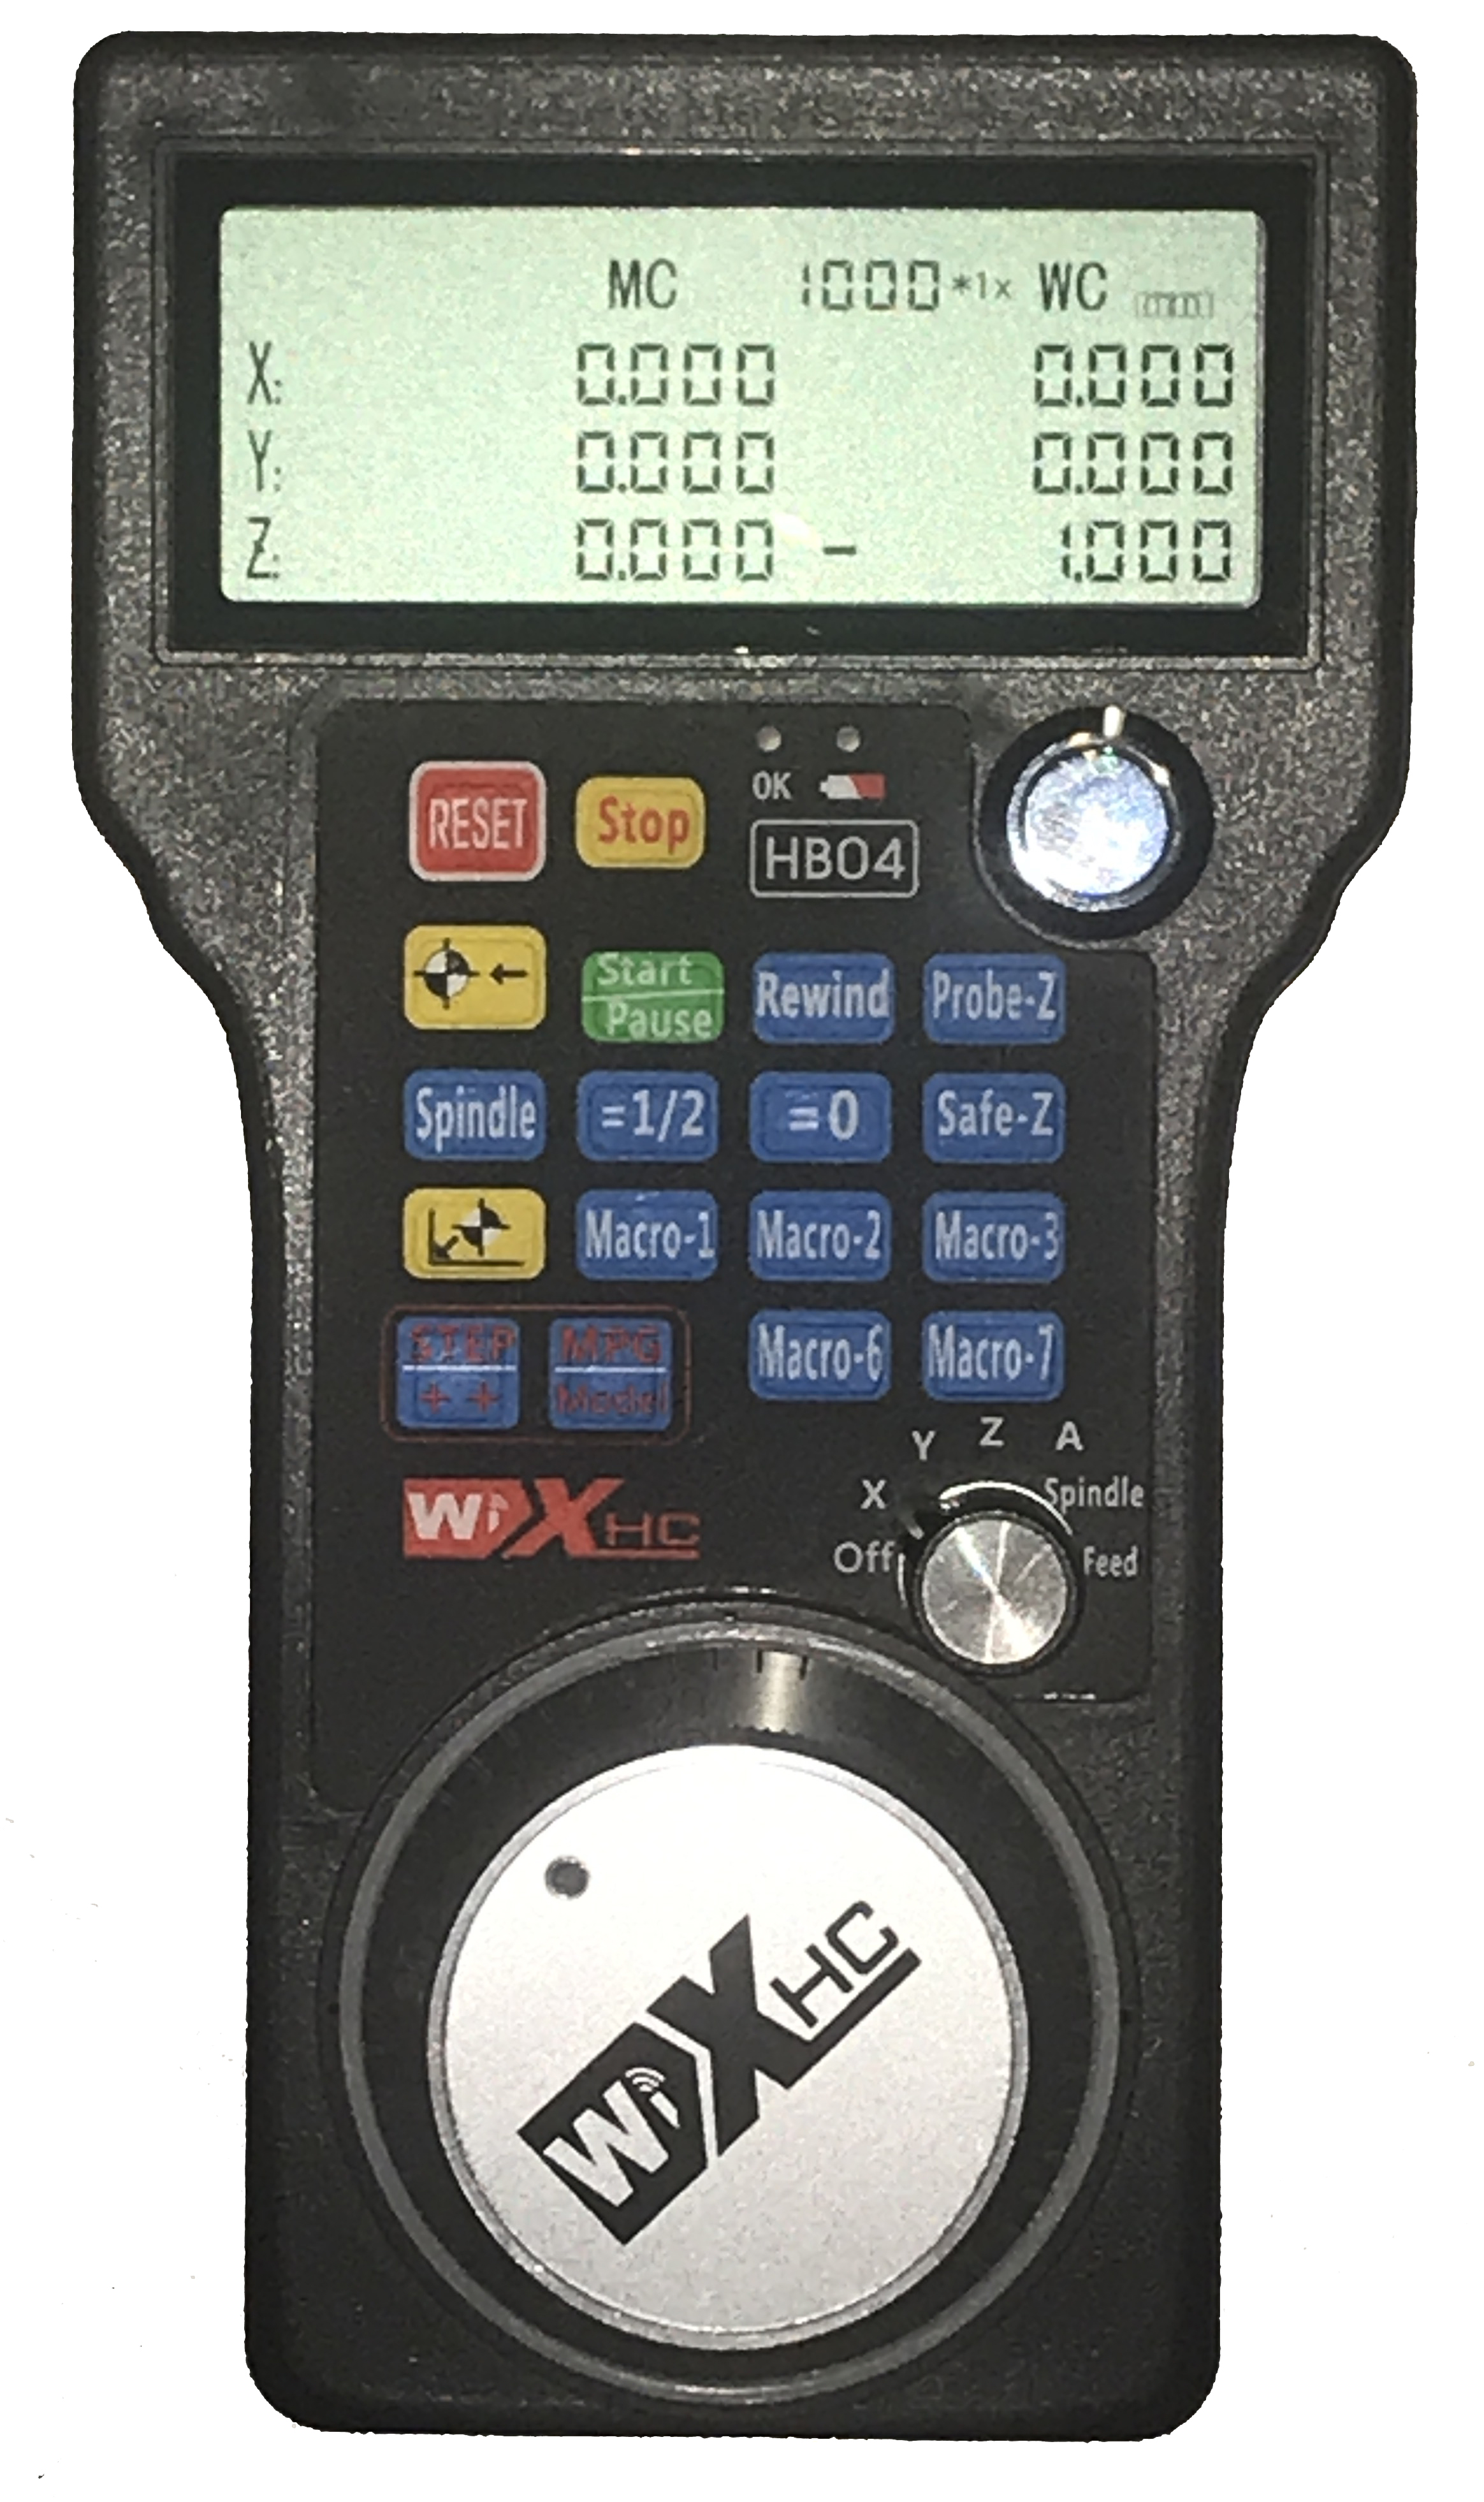
\includegraphics[scale=0.05]{whb04.jpg}
    \caption{WHB04 Pendant/MPG  }
    \label{fig:whb04}
    \end{figure}

 

\subsection{WHB04 Controls}

Figure~\ref{fig:whb04-keypad} shows a close up of the WHB keypad.

The two main controls of the MPG are the small axis selector knob  you can see in the closeup 
and the large pulse wheel.

In general the axis selector selects which axis or other parameter is affected
by the pulse wheel or buttons on the keypad. 
 
For some functions setting the selector knob to 'Off' will make those functions
apply to all axes at once.

\begin{figure}[htb]
    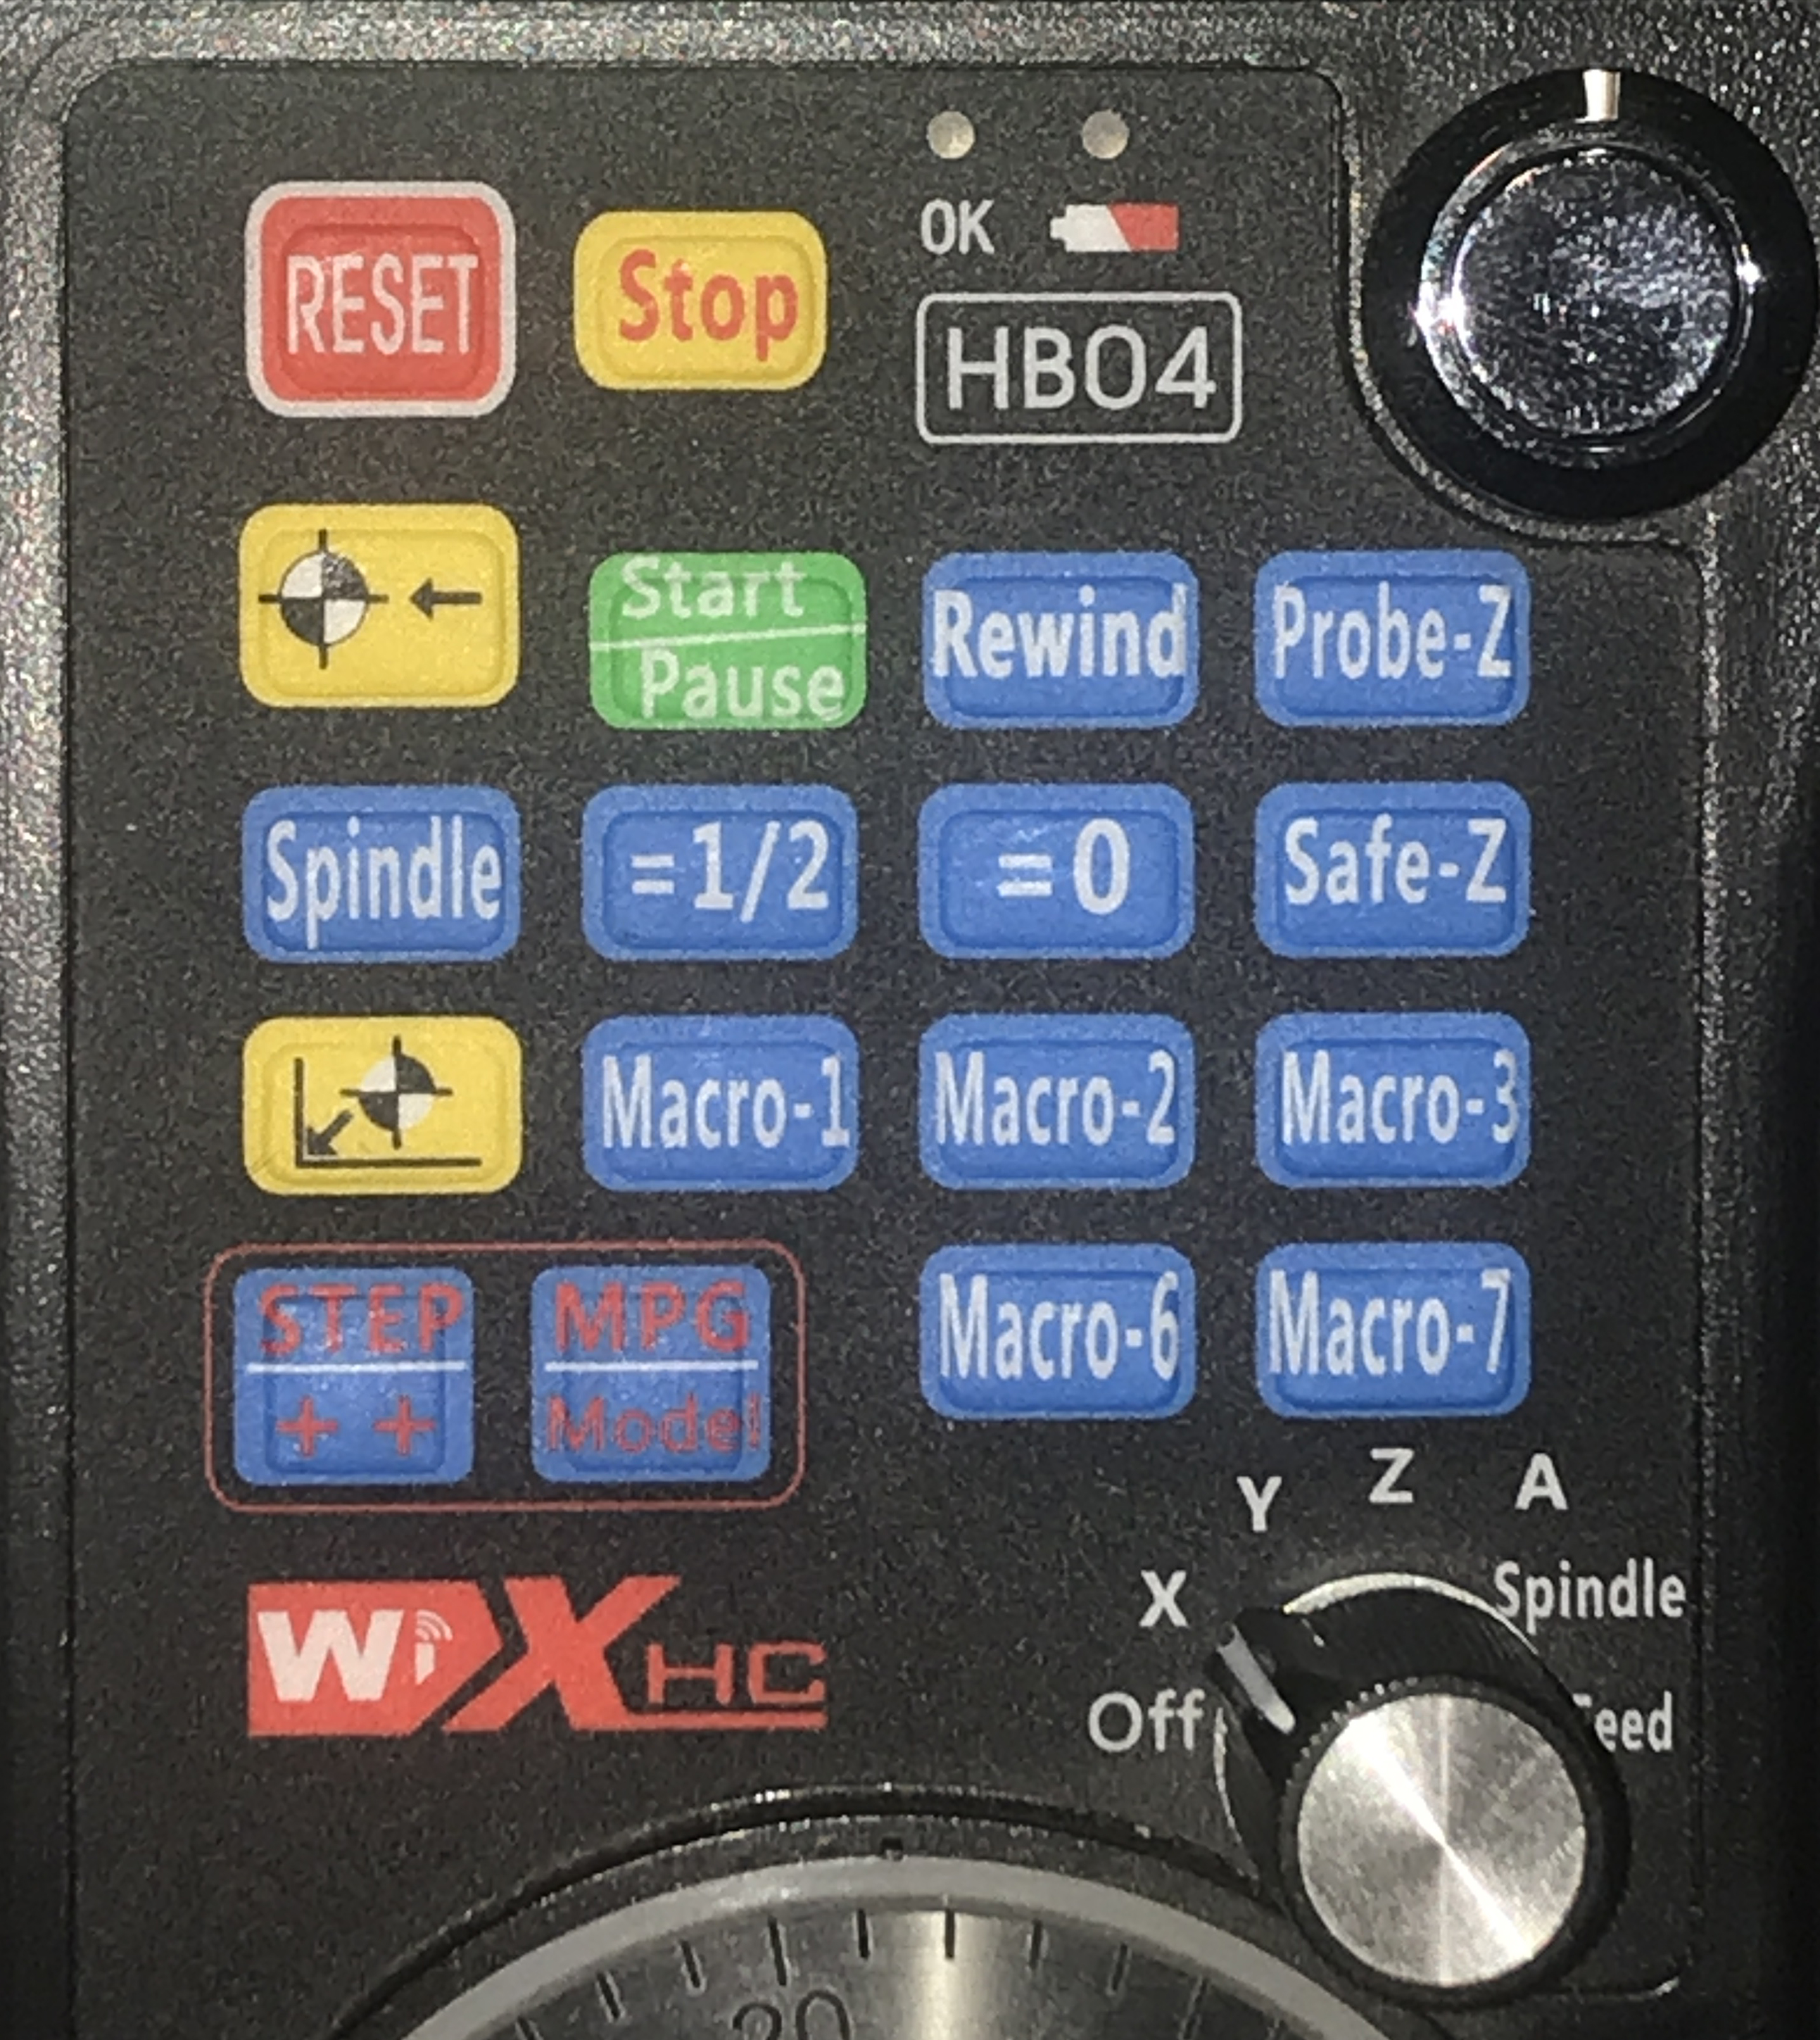
\includegraphics[scale=0.10]{whb04-keypad.jpg}
    \caption{WHB03 Keypad}
    \label{fig:whb04-keypad}
    \end{figure}


\subsection{WHB04 Display}

Figure~\ref{fig:whb04-display} shows a close up of the WHB04 display.

The display has DROs for three axes at a time. If the axis selector
is in X,Y or Z position then the corresponding axis values are 
displayed in the DROs. If the selector is in A position then axis positions
of the A, B and C axis are displayed.

The DROs in the 'MC' column are not used (to avoid confusion) and always display'0.000'

The DROs in the 'WC' column display the same DRO values as on the EazyCNC computer screen.

Note that you can NOT see more decimals on the pendant DRO than on the computer screen 
eventhough the pendant always displays three digits.

Next to the WC text to the right an 'inch' or 'mm' sign is show and reflects 
weather the DRO values and wheel operate in inch or mm mode. This is controlled
by the units selected for the DROs in EazyCNC.
   
%---------------------------------------------------------------------------
\begin{figure}[htb]
    \includegraphics[scale=0.]{whb04-display.jpg}
    \caption{WHB04 Display }
    \label{fig:whb04-display}
    \end{figure}

\subsection{WHB04 Wheel}


Every 'click' of the wheel moves the selected axis one step to the wheel direction.
The speed at which the mill table,head or plasma torch moves is relative to how fast you
turn the wheel. 

In principle the wheel allows absolute (well incremental really) control of 
the axis position and speed. In practice the wheel sometimes misses pulses 
so turning the wheel ten clicks may only result in nine steps, always
confirm by looking at the DROs.

Because it is possible to turn the wheel faster than the axis can move there
is a windup prevention that prevents the wheel position from advancing too 
much beyond where the axis has advanced.

Because of the long chain of hardware and software that connects the pulse wheel
to the axis stepper motor, the feel of control you get with the wheel is far from 
perfect. However it does allow you to control the axis position rather
swiftly and accurately.

The 'step size' i.e. how much every wheel click moves milling table is displayed
to the left of the 'WC' text. It is expressed as number of 1/1000th of the 
units selected for the DROs. Very much like the jogging step selection but 
separate from that.

In 'mm' mode the displayed text and step size are as follows:

\begin{tabular}{ r | l }
x1000 &  1.000 mm \\
x100  &  0.100 mm \\
x10  &   0.010 mm \\
x0   &   1 stepper step \\
\end{tabular}

In 'inch' mode the displayed text and step size are as follows:

\begin{tabular}{ r | l }
x100  & 0.100 inch \\
x10   & 0.010 inch \\
x1    & 0.001 inch \\
x0   &   1 stepper step \\
\end{tabular}

You change the step size with the 'STEP++' key, see below.

\seticons{whb04-step-button}
\subsection{Step++ -key}       
   
Pressing this key shortly will advance the step size to the next \emph{smaller}
size. After 'x0' the step size reverts to the largest steps size ('x1000'
for 'mm mode and 'x100' for 'inch' mode).

A long press (over 1 seconds) will revert the step size tolargest steps size.

Whenever the largest step size is selected a long 'beep' sound is emitted
from the computer to alert the user.

\seticons{whb04-auto-touch-xy-button}
\subsection{Probe XY -key}  


Pressing this key has the same effect as 
pressing the -X or -Y Touch button in the Work Offsets screen when the 
'Use PROBE to Touch' feature is enabled.

In other word this will perform a short probing move on the selected 
axis and as soon as the probe trips the movement stops and rectracts 
and the selected axis work offset is set to the negative half value of 
the Probe Diameter parameter in 
the Work Offsets screen.

Thus this is a handy way to perform edge finding using a probe and the MPG.

Use the axis selector knog to select either X or Y axis. You can only
probe on the left/front side of the work piece with this key.

\seticons{whb04-probe-z-button}
\subsection{'Probe Z' -key}       
 
Pressing this key has the same effect as 
pressing the Touch button in the Work Offsets / Set Z origin screen when the 
'Use PROBE to Touch' feature is enabled.
    
In other word this will perform a short probing move on the Z axis 
axis and as soon as the probe trips the movement stops and rectracts 
and the Z axis work offset is set to the Gage Height parameter in 
the Work Offsets screen.
    
Thus this is a handy way to perform 'zero' the Z-axis with the probe.
    

\seticons{whb04-spindle-button}
\subsection{Spindle -key}  

Pressing this key has the same effect as pressing the SPINDLE button on 
the computer screen. 

In other words it toggles the spindle on and off.

\seticons{whb04-start-pause-button}
\subsection{Start/Pause -key}  

This key has the same effect as pressing alternatively the RUN and HOLD buttons
on the computer screen.

\seticons{whb04-stop-button}
\subsection{Stop -Key}       

This key has the same effect as pressing the STOP button on the computer screen.
 
\seticons{whb04-half-button}
\subsection{'=1/2' -key}       

Pressing this key has the same effect as 
pressing the Touch -X or Touch -Y  button in the Work Offsets screen when the 
'Use PROBE to Touch' feature is NOT enabled.
    
In other words the selected axis Work Offset is set to the negative half value of the Probe Diameter parameter in 
the Work Offsets screen.
    
Thus this is a handy way to perform edge finding manually with 
an edge finder and the MPG.
    
Use the axis selector knog to select either X or Y axis. You can only
Touch on the left/front side of the work piece with this key.
            
\seticons{whb04-goto-origin-button}     
\subsection{'Goto Origin' -key}       
       
Pressing this key will cause the X and Y axis to jog to the zero
position of the DROs.


\seticons{whb04-zero-button}     
\subsection{'=0' -key}       

Pressing this key has the same effect as 
pressing the ZERO button in the selected axis.

Use the axis selector knob to select the affected axis, or set the
axis selector knob to 'Off' to ZERO all axis.

\seticons{whb04-safe-z-button}          
\subsection{Safe Z -key}       

                                              
Pressing this key will cause the Z-axis to move to the 
Safe Z value set in the Axis Setup / Axis Z.

\seticons{whb04-reset-button}
\subsection{Reset -key}       

                                              
Pressing this has the same effect as pressing HOME button on the computer 
screen.

Use the axis selector knob to select the affected axis, or set the
axis selector knob to 'Off' to HOME ALL axis.

A long press will force HOME ALL action regardless of the axis selector knob position.


\seticons{whb04-rewind-button}
\subsection{Rewind -key}       

Pressing this key will change the currently selected tool to the next tool number, 
in other words this has the same effect as L-word in G-code. Note that it does
not actually cause any tool change but does effect the tool offset, if it is 
enabled with G43 code.

Long press will reset the current tool to tool number 1. 

Whenever the tool number1 is selected  a long 'beep' sound is emitted
from the computer to alert the user.

This key is mainly intended to help setting up tool length without touching
the computer keyboard.






\newcommand{\noicons}{\savebox{\iconbox}{}}
\noicons



\section{XHC WHB04B Pendant / MPG} 
\begin{figure}[htb]
\includegraphics[scale=0.07]{whb04b.jpg}
\caption{WHB04B Pendant / MPG}
\label{fig:whb04b}
\end{figure}

EazyCNC supports a commercially available MPG named WHB04B 
(note the B at then end of the type code), 
see Figure~\ref{fig:whb04b}.  This actually comes in two varieties, 
WHB04B-4 for use with four axis and WHB04B-6 for use with six axis.
    
Out of the box this pendant (or rather EazyCNC) support a
much smaller set of functionality than for example the WHB04.
This is because the pendant has a smaller number of buttons
and even smaller number of usefully labeled buttons.

\subsection{WHB04B Controls}


The three main controls of the MPG are the axis selector knob,
step size selector knob and the large pulse wheel.

In general the axis selector selects which axis is affected
by the pulse wheel or buttons on the keypad. 
 
The step size selector change how fast the wheel moves the axis.

The keypad is used to activate EazyCNC functions.

\subsection{Display}
\begin{figure}[htb]
\includegraphics[scale=0.2]{whb04b-display.jpg}
\caption{WHB04B Display}
\label{fig:whb04b-display}
\end{figure}

Figure~\ref{fig:whb04b-display} shows a close up of the WHB04B display.

The display has DROs for three axes at a time. If the axis selector
is in X,Y or Z position then the corresponding axis values are 
displayed in the DROs. If the selector is in A position then axis positions
of the A, B and C axis are displayed.

An asterisk ('*') in front of an axis letter indicates that that axis has
is currently selected by the Axis Selector knob.
    
The DROs  display the same DRO values as on the EazyCNC computer screen.
    
Note that you can NOT see more decimals on the pendant DRO than on the computer screen 
eventhough the pendant always displays four decimal digits.
    
Note that if the Axis Selector is in the OFF position then EazyCNC
is not able to update the display at all.

On the top row alternatively eithe step selector percentage is displayed
or feed  ('F') or spindle ('S') is displayed. The percentage makes
little sense but can be used as a reminder of the selected wheel step size.

To display the feed or spindle speed you need to press the Feed +/- or 
Spindle +/- key. If the corrosponding feed or spindle speed is not 
currently displaying when you press the key then the display will switch
and the key is ignored, i.e. it will not change the feed or spindle speed.

When the pendant is powered up you may see the text 'RESET' on the top row.
To get rid of that you have to press any button on the key pad and rotate
the step selector knob. This is makes no sense but it is what it is
and EazyCNC cannot do anything about that.




\subsection{Keypad}
\begin{figure}[htb]
\includegraphics[scale=0.2]{whb04b-keypad.jpg}
\caption{WHB04B Keypad}
\label{fig:whb04b-keypad}
\end{figure}

Figure~\ref{fig:whb04b-keypad} shows a close up of the WHB04B keypad.

The keypad has 15 keys plus the orange 'Fn' key which alter the
functions of those keys that have an orange label on them. To 
activate the 'orange' function you need to hold the 'Fn' key down
while pressing the intended key.

Note that the functions associated with the keys are not fixed
and you can change them
in the Mach Setup / Shortcuts screen, see section \ref{sec:shortcut-setup},

For inspiration of functions you could assign to the keys I suggest
reading the WHB04 appendix which lists number of useful functions
that are available out-of-the-box with that pendant.



\subsection{Axis Selector}
\begin{figure}[htb]
\includegraphics[scale=0.2]{whb04b-axis-knob.jpg}
\caption{WHB04B Axis Selector }
\label{fig:whb04b-axis-knob}
\end{figure}



\subsection{WHB04 Wheel}

Every 'click' of the wheel moves the selected axis one step to the wheel direction.
The speed at which the mill table,head or plasma torch moves is relative to how fast you
turn the wheel. 
    
In principle the wheel allows absolute (well incremental really) control of 
the axis position and speed. In practice the wheel sometimes misses pulses 
so turning the wheel ten clicks may only result in nine steps, always
confirm by looking at the DROs.
    
Because it is possible to turn the wheel faster than the axis can move there
is a windup prevention that prevents the wheel position from advancing too 
much beyond where the axis has advanced.
    
Because of the long chain of hardware and software that connects the pulse wheel
to the axis stepper motor, the feel of control you get with the wheel is far from 
perfect. However it does allow you to control the axis position rather
swiftly and accurately.

The step size that is used when you turn the wheel depends on the Step Selector, 
see below.
    
\subsection{Step Selector}
\begin{figure}[htb]
\includegraphics[scale=0.2]{whb04b-step-knob.jpg}
\caption{WHB04B Step Selector}
\label{fig:whb04b-step-knob}
\end{figure}

The Step Selector has some confusing labeling, you should go by the
labels in white.

Depending on weather you are working with  inches or millimeters 
(see Mach Setup / Screen / Units)
the wheel click/step size varies as shown in the table below. 

\begin{tabular}{ r | l | l }
Selector position& Units = mm & Units = inch\\
\hline
0.001 / 2\% &  0.001 mm  & 0.001" (0.0254 mm)\\
0.01 / 5\% &  0.01 mm  & 0.001" (0.254 mm)\\
0.1 / 10\% &  0.1 mm  & 0.001" (2.54 mm)\\
1.0 / 30\% &  1.0 mm  & minimal\\
LEAD\% &  minimal  & minimal\\
\end{tabular}
    
In above 'minimal' indicates smallest possible step, for example
if in your Axis Setup / Step/mm you have 400 step/mm then 
the minimal step size is 1/400 mm i.e. 0.0025 mm.

Note that if theoretical step size as per above table results
in a step that is smaller than 'minimal' then the minimal step is 
selected.

For safety the "1.0" selector position does not result in one 
inch step size in inch mode. 

\seticons{whb04b-reset}
\subsection{Reset -Key}   
                                  
Pressing this has the same effect as pressing HOME button on the computer 
screen.

Use the axis selector knob to select the affected axis, or set the
axis selector knob to 'Off' to HOME ALL axis.

A long press will force HOME ALL action regardless of the axis selector knob position.


\seticons{whb04b-stop}
\subsection{Stop -Key}  


This key has the same effect as pressing the STOP button on the computer screen.
 
\seticons{whb04b-start-pause}
\subsection{Start / Run -key}   
 
This key has the same effect as pressing alternatively the RUN and HOLD buttons
on the computer screen.
   


\seticons{whb04b-feed+}
\subsection{Macro-1 [Feed+]-key} 

If the 'F' is not displayed on the pendant display then the key press 
is ignored and the display changes to display the feed speed.

When pressed together with the 'Fn' key this button has the same effect
as pressing the '+' key in the Feed/Override panel on the screen.

When pressed without  the 'Fn' key this key has no function unless you
assign one to it.
    

\seticons{whb04b-feed-}
\subsection{Macro-2 [Feed-]-key}   


If the 'F' is not displayed on the pendant display then the key press 
is ignored and the display changes to display the feed speed.

When pressed together with the 'Fn' key this button has the same effect
as pressing the '-' key in the Feed/Override panel on the screen.

When pressed without  the 'Fn' key this key has no function unless you
assign one to it.
  
\seticons{whb04b-spindle+}
\subsection{Macro-3 [Spindle+] -key}   


If the 'S' is not displayed on the pendant display then the key press 
is ignored and the display changes to display the spindle speed.

When pressed together with the 'Fn' key this button has the same effect
as pressing the '+' key in the Spindle panel on the screen.

When pressed without  the 'Fn' key this key has no function unless you
assign one to it.
  

\seticons{whb04b-spindle-}
\subsection{Macro-4 [Spindle-]-key}  


If the 'S' is not displayed on the pendant display then the key press 
is ignored and the display changes to display the spindle speed.

When pressed together with the 'Fn' key this button has the same effect
as pressing the '-' key in the Spindle panel on the screen.

When pressed without  the 'Fn' key this key has no function unless you
assign one to it.

\seticons{whb04b-m-home}
\subsection{Macro-5 [M-HOME]-key}   

This key has no function unless you assign one to it.

\seticons{whb04b-safe-z}
\subsection{Macro-6 [Safe-Z]-key}    
    
                                              
Pressing this key will cause the Z-axis to move to the  Safe Z value set in the Axis Setup / Axis Z.


\seticons{whb04b-w-home}
\subsection{Macro-7 [W-HOME]-key}

Pressing this key will cause the X and Y axis to jog to the zero
position of the DROs.

    
\seticons{whb04b-s-on-off}
\subsection{Macro-8 [S-ON/OFF]-key}  

Pressing this key has the same effect as pressing the SPINDLE button on 
the computer screen. 

In other words it toggles the spindle on and off.


\seticons{whb04b-fn}
\subsection{Fn -key}       
 
This key together with some other is used to evoke the secondary 
function of that key. To use that press and hold the 'Fn' key down
while pressing the other key.
    
\seticons{whb04b-probe-z}
\subsection{Macro-9 [Probe-Z]-key}   


Pressing this key has the same effect as 
pressing the Touch button in the Work Offsets / Set Z origin screen when the 
'Use PROBE to Touch' feature is enabled.
    
In other word this will perform a short probing move on the Z axis 
axis and as soon as the probe trips the movement stops and rectracts 
and the Z axis work offset is set to the Gage Height parameter in 
the Work Offsets screen.
    
Thus this is a handy way to perform 'zero' the Z-axis with the probe.
 
\seticons{whb04b-macro-10}
\subsection{Macro-10}   


This key has no function unless you assign one to it.

\seticons{whb04b-continuous}
\subsection{Continuous -key}  


This key has no function unless you assign one to it.

\seticons{whb04b-step}
\subsection{Step -key}       

This key has no function unless you assign one to it.





% firmware description
% mechanical construction

%mains
%probe 
%no jumpers, just wires



\clearpage
\thispagestyle{empty}
\vspace*{\fill}
\begin{center} 
{ \huge \bfseries ***  The End *** }
\vspace*{\fill}
\end{center}

\end{document}  
